\chapter{Particular Presets} 
\lstset{style=6502Style}

\clearpage                                                                 
\begin{figure}[H]                                                          
    \centering                                                             
    \begin{adjustbox}{width=14cm,center}                                   
      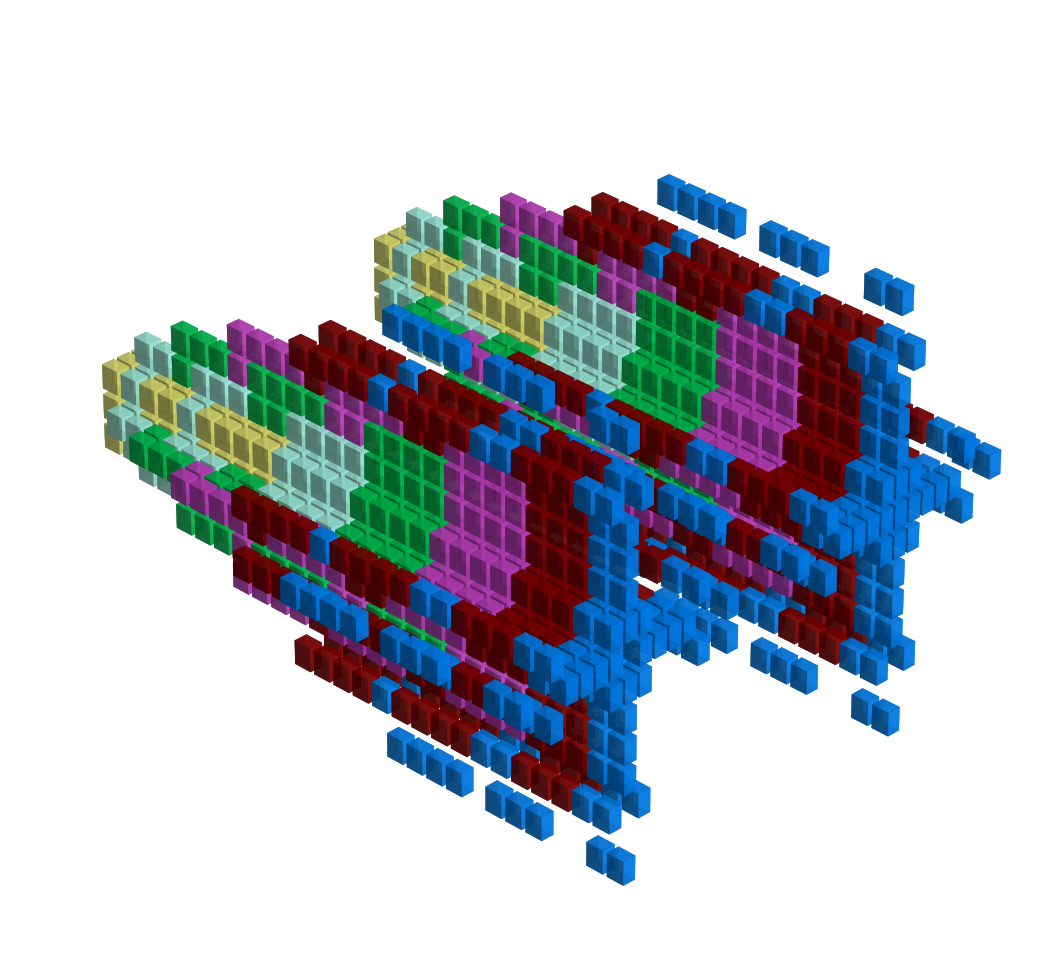
\includegraphics[width=14cm]{src/presets/pattern0-45.png}%           
    \end{adjustbox}                                                        
\caption{Evolution of Preset 0.}                                           
\end{figure}                                                               
\clearpage                                                                 
                                                                           
\begin{lstlisting}[basicstyle=\tiny,caption=Source code for Preset 0.]
preset0
        ; unusedPresetByte: Unused Byte
        .BYTE $00
        ; smoothingDelay: 'Because of the time taken to draw larger patterns speed
        ; increase/decrease is not linear. You can adjust the 'compensating delay'
        ; which often smooths out jerky patterns. Can be used just for special FX),
        ; though. Suck it and see.'
        .BYTE $0C
        ; cursorSpeed: 'Gives you a slow or fast little cursor, according to setting.'
        .BYTE $02
        ; bufferLength: 'Larger patterns flow more smoothly with a shorter
        ; Buffer Length - not so many positions are retained so less plotting to do.
        ; Small patterns with a long Buffer Length are good for 'steamer' effects.
        ; N.B. Cannot be adjusted whilst patterns are actually onscreen.'
        .BYTE $1F
        ; pulseSpeed: 'Usually if you hold down the button you get a continuous
        ; stream. Setting the Pulse Speed allows you to generate a pulsed stream, as
        ; if you were rapidly pressing and releasing the FIRE button.'
        .BYTE $01
        ; indexForColorBarDisplay: 'The initial index for the color displayed
        ; in the color bar when adjusting the colors for each step.'
        .BYTE $01
        ; lineWidth: 'Sets the width of the lines produced in Line Mode.'
        .BYTE $07
        ; sequencerSpeed: 'Controls the rate at which sequencer feeds in its data. '
        .BYTE $04
        ; pulseWidth: 'Sets the length of the pulses in a pulsed stream output.
        ; Don't worry about what that means - just get in there and mess with it.'
        .BYTE $01
        ; baseLevel: 'Controls how many 'levels' of pattern are plotted.'
        .BYTE $07
        ; presetColorValuesArray: 'Allows you to set the colour for each of the
        ; seven pattern steps. Set up the colour you want, press RETURN, and the
        ; command offers the next colour along, up to no. 7, then ends. Cannot be
        ; adjusted while patterns being generated.'
        .BYTE BLACK,BLUE,RED,PURPLE,GREEN,CYAN,YELLOW,WHITE
        ; trackingActivated: 'Controls whether logic-seeking is used in the
        ; buffer or not. The upshot of this for you is a slightly different feel -
        ; continuous but fragmented when ON, or together-ish bursts when OFF. Try it.'
        .BYTE $00
        ; lineModeActivated: 'A bit like drawing with the Aurora Borealis'
        .BYTE $00
        ; presetIndex: 'This calls in one of the 16 presets, stored Lightsynth
        ; parameters which give different effects. Try them all out io see some uf
        ; the multitude of effects which you cai achieve using the system. Some are
        ; fast, some slow, some pulse, others swirl. Play with them all, try them to
        ; different music.'
        .BYTE $00
        ; currentPatternElement: 'Initial pattern used by this preset.'
        .BYTE $00
        ; currentSymmetrySetting: 'Current symmetry setting.'
        ; Possible values are 0 - 4:
        ; 'NO SYMMETRY     '
        ; 'Y-AXIS SYMMETRY '
        ; 'X-Y SYMMETRY    '
        ; 'X-AXIS SYMMETRY '
        ; 'QUAD SYMMETRY   '
        .BYTE $01
        ; Unused Data.
        .BYTE $FF,$00,$FF,$FF,$00,$FF,$00,$FF,$00
\end{lstlisting}


\clearpage                                                                 
\begin{figure}[H]                                                          
    \centering                                                             
    \begin{adjustbox}{width=14cm,center}                                   
      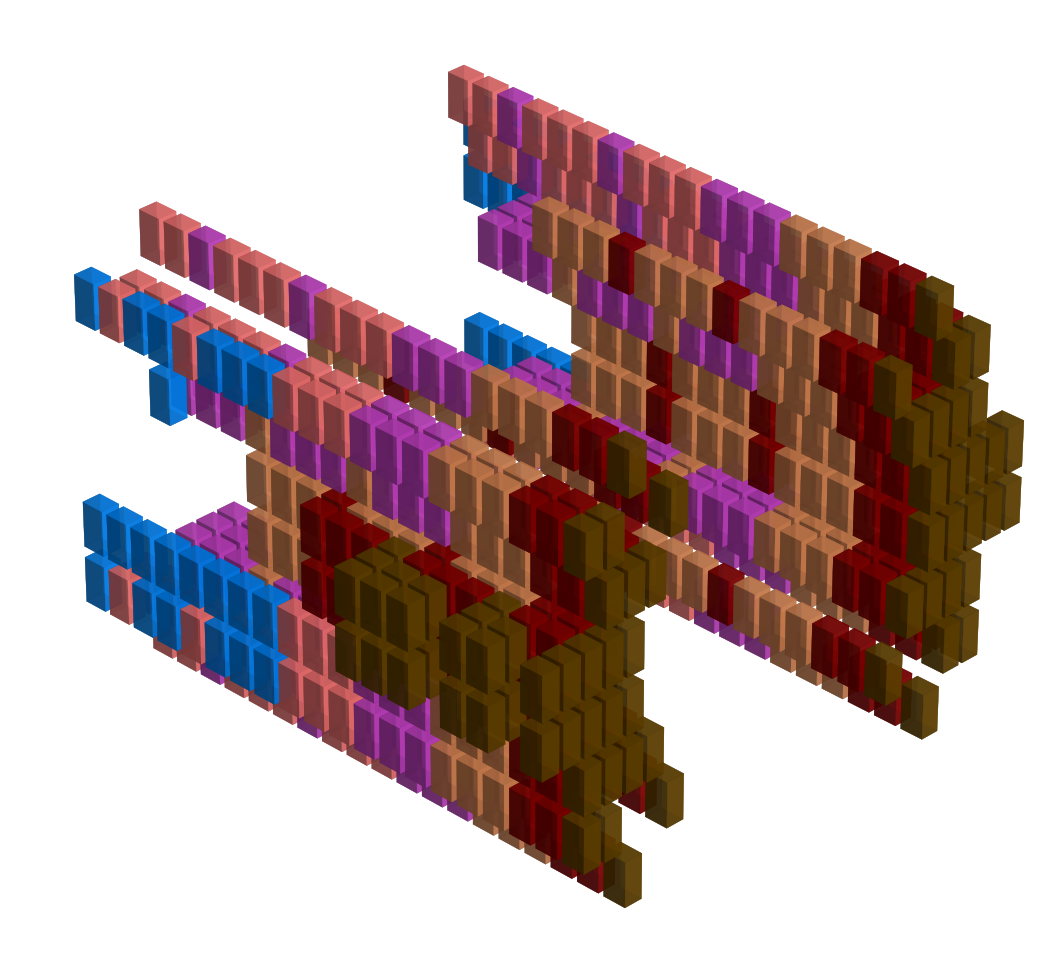
\includegraphics[width=14cm]{src/presets/pattern1-45.png}%           
    \end{adjustbox}                                                        
\caption{Evolution of Preset 1.}                                           
\end{figure}                                                               
\clearpage                                                                 
                                                                           
\begin{lstlisting}[basicstyle=\tiny,caption=Source code for Preset 1.]
preset1
        ; unusedPresetByte: Unused Byte
        .BYTE $00
        ; smoothingDelay: 'Because of the time taken to draw larger patterns speed
        ; increase/decrease is not linear. You can adjust the 'compensating delay'
        ; which often smooths out jerky patterns. Can be used just for special FX),
        ; though. Suck it and see.'
        .BYTE $0C
        ; cursorSpeed: 'Gives you a slow or fast little cursor, according to setting.'
        .BYTE $02
        ; bufferLength: 'Larger patterns flow more smoothly with a shorter
        ; Buffer Length - not so many positions are retained so less plotting to do.
        ; Small patterns with a long Buffer Length are good for 'steamer' effects.
        ; N.B. Cannot be adjusted whilst patterns are actually onscreen.'
        .BYTE $28
        ; pulseSpeed: 'Usually if you hold down the button you get a continuous
        ; stream. Setting the Pulse Speed allows you to generate a pulsed stream, as
        ; if you were rapidly pressing and releasing the FIRE button.'
        .BYTE $01
        ; indexForColorBarDisplay: 'The initial index for the color displayed
        ; in the color bar when adjusting the colors for each step.'
        .BYTE $0E
        ; lineWidth: 'Sets the width of the lines produced in Line Mode.'
        .BYTE $07
        ; sequencerSpeed: 'Controls the rate at which sequencer feeds in its data. '
        .BYTE $08
        ; pulseWidth: 'Sets the length of the pulses in a pulsed stream output.
        ; Don't worry about what that means - just get in there and mess with it.'
        .BYTE $01
        ; baseLevel: 'Controls how many 'levels' of pattern are plotted.'
        .BYTE $07
        ; presetColorValuesArray: 'Allows you to set the colour for each of the
        ; seven pattern steps. Set up the colour you want, press RETURN, and the
        ; command offers the next colour along, up to no. 7, then ends. Cannot be
        ; adjusted while patterns being generated.'
        .BYTE BLACK,BROWN,RED,ORANGE,PURPLE,LTRED,BLUE,LTBLUE
        ; trackingActivated: 'Controls whether logic-seeking is used in the
        ; buffer or not. The upshot of this for you is a slightly different feel -
        ; continuous but fragmented when ON, or together-ish bursts when OFF. Try it.'
        .BYTE $FF
        ; lineModeActivated: 'A bit like drawing with the Aurora Borealis'
        .BYTE $00
        ; presetIndex: 'This calls in one of the 16 presets, stored Lightsynth
        ; parameters which give different effects. Try them all out io see some uf
        ; the multitude of effects which you cai achieve using the system. Some are
        ; fast, some slow, some pulse, others swirl. Play with them all, try them to
        ; different music.'
        .BYTE $01
        ; currentPatternElement: 'Initial pattern used by this preset.'
        .BYTE $01
        ; currentSymmetrySetting: 'Current symmetry setting.'
        ; Possible values are 0 - 4:
        ; 'NO SYMMETRY     '
        ; 'Y-AXIS SYMMETRY '
        ; 'X-Y SYMMETRY    '
        ; 'X-AXIS SYMMETRY '
        ; 'QUAD SYMMETRY   '
        .BYTE $04
        ; Unused Data.
        .BYTE $FF,$00,$FF,$FF,$00,$FF,$00,$FF,$00
\end{lstlisting}


\clearpage                                                                 
\begin{figure}[H]                                                          
    \centering                                                             
    \begin{adjustbox}{width=14cm,center}                                   
      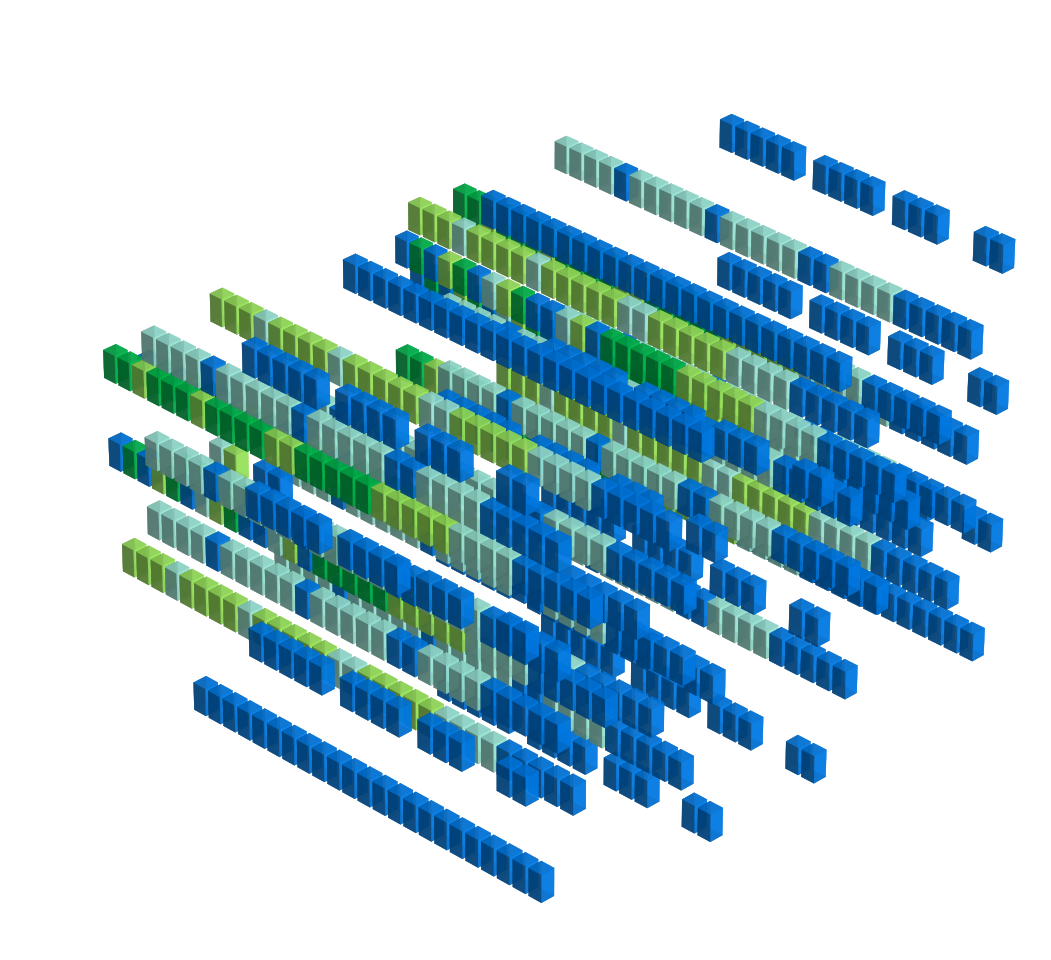
\includegraphics[width=14cm]{src/presets/pattern2-45.png}%           
    \end{adjustbox}                                                        
\caption{Evolution of Preset 2.}                                           
\end{figure}                                                               
\clearpage                                                                 
                                                                           
\begin{lstlisting}[basicstyle=\tiny,caption=Source code for Preset 2.]
preset2
        ; unusedPresetByte: Unused Byte
        .BYTE $00
        ; smoothingDelay: 'Because of the time taken to draw larger patterns speed
        ; increase/decrease is not linear. You can adjust the 'compensating delay'
        ; which often smooths out jerky patterns. Can be used just for special FX),
        ; though. Suck it and see.'
        .BYTE $0B
        ; cursorSpeed: 'Gives you a slow or fast little cursor, according to setting.'
        .BYTE $02
        ; bufferLength: 'Larger patterns flow more smoothly with a shorter
        ; Buffer Length - not so many positions are retained so less plotting to do.
        ; Small patterns with a long Buffer Length are good for 'steamer' effects.
        ; N.B. Cannot be adjusted whilst patterns are actually onscreen.'
        .BYTE $28
        ; pulseSpeed: 'Usually if you hold down the button you get a continuous
        ; stream. Setting the Pulse Speed allows you to generate a pulsed stream, as
        ; if you were rapidly pressing and releasing the FIRE button.'
        .BYTE $01
        ; indexForColorBarDisplay: 'The initial index for the color displayed
        ; in the color bar when adjusting the colors for each step.'
        .BYTE $01
        ; lineWidth: 'Sets the width of the lines produced in Line Mode.'
        .BYTE $07
        ; sequencerSpeed: 'Controls the rate at which sequencer feeds in its data. '
        .BYTE $0B
        ; pulseWidth: 'Sets the length of the pulses in a pulsed stream output.
        ; Don't worry about what that means - just get in there and mess with it.'
        .BYTE $01
        ; baseLevel: 'Controls how many 'levels' of pattern are plotted.'
        .BYTE $07
        ; presetColorValuesArray: 'Allows you to set the colour for each of the
        ; seven pattern steps. Set up the colour you want, press RETURN, and the
        ; command offers the next colour along, up to no. 7, then ends. Cannot be
        ; adjusted while patterns being generated.'
        .BYTE BLACK,BLUE,LTBLUE,CYAN,LTGREEN,GREEN,LTBLUE,BLUE
        ; trackingActivated: 'Controls whether logic-seeking is used in the
        ; buffer or not. The upshot of this for you is a slightly different feel -
        ; continuous but fragmented when ON, or together-ish bursts when OFF. Try it.'
        .BYTE $FF
        ; lineModeActivated: 'A bit like drawing with the Aurora Borealis'
        .BYTE $00
        ; presetIndex: 'This calls in one of the 16 presets, stored Lightsynth
        ; parameters which give different effects. Try them all out io see some uf
        ; the multitude of effects which you cai achieve using the system. Some are
        ; fast, some slow, some pulse, others swirl. Play with them all, try them to
        ; different music.'
        .BYTE $05
        ; currentPatternElement: 'Initial pattern used by this preset.'
        .BYTE $05
        ; currentSymmetrySetting: 'Current symmetry setting.'
        ; Possible values are 0 - 4:
        ; 'NO SYMMETRY     '
        ; 'Y-AXIS SYMMETRY '
        ; 'X-Y SYMMETRY    '
        ; 'X-AXIS SYMMETRY '
        ; 'QUAD SYMMETRY   '
        .BYTE $01
        ; Unused Data.
        .BYTE $FF,$00,$FF,$FF,$00,$FF,$00,$FF,$00
\end{lstlisting}


\clearpage                                                                 
\begin{figure}[H]                                                          
    \centering                                                             
    \begin{adjustbox}{width=14cm,center}                                   
      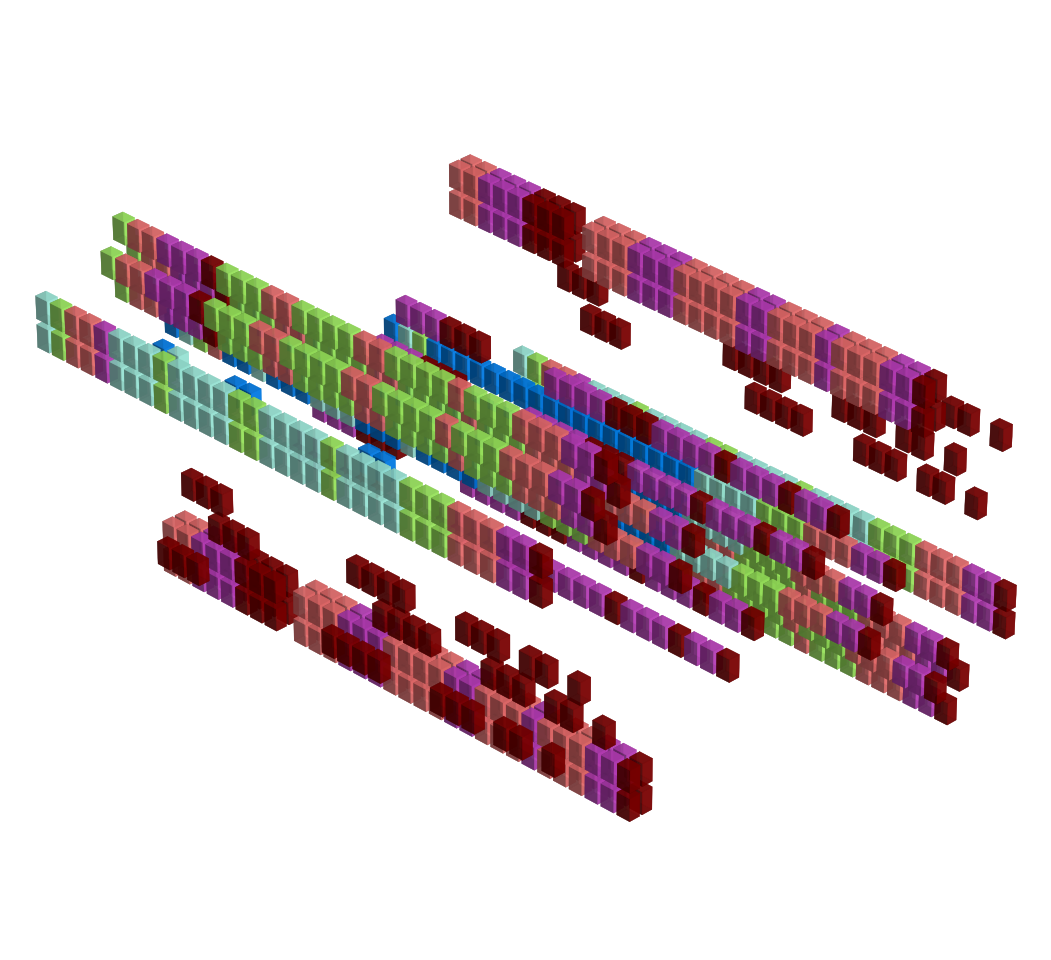
\includegraphics[width=14cm]{src/presets/pattern3-45.png}%           
    \end{adjustbox}                                                        
\caption{Evolution of Preset 3.}                                           
\end{figure}                                                               
\clearpage                                                                 
                                                                           
\begin{lstlisting}[basicstyle=\tiny,caption=Source code for Preset 3.]
preset3
        ; unusedPresetByte: Unused Byte
        .BYTE $00
        ; smoothingDelay: 'Because of the time taken to draw larger patterns speed
        ; increase/decrease is not linear. You can adjust the 'compensating delay'
        ; which often smooths out jerky patterns. Can be used just for special FX),
        ; though. Suck it and see.'
        .BYTE $04
        ; cursorSpeed: 'Gives you a slow or fast little cursor, according to setting.'
        .BYTE $02
        ; bufferLength: 'Larger patterns flow more smoothly with a shorter
        ; Buffer Length - not so many positions are retained so less plotting to do.
        ; Small patterns with a long Buffer Length are good for 'steamer' effects.
        ; N.B. Cannot be adjusted whilst patterns are actually onscreen.'
        .BYTE $26
        ; pulseSpeed: 'Usually if you hold down the button you get a continuous
        ; stream. Setting the Pulse Speed allows you to generate a pulsed stream, as
        ; if you were rapidly pressing and releasing the FIRE button.'
        .BYTE $01
        ; indexForColorBarDisplay: 'The initial index for the color displayed
        ; in the color bar when adjusting the colors for each step.'
        .BYTE $01
        ; lineWidth: 'Sets the width of the lines produced in Line Mode.'
        .BYTE $07
        ; sequencerSpeed: 'Controls the rate at which sequencer feeds in its data. '
        .BYTE $0A
        ; pulseWidth: 'Sets the length of the pulses in a pulsed stream output.
        ; Don't worry about what that means - just get in there and mess with it.'
        .BYTE $01
        ; baseLevel: 'Controls how many 'levels' of pattern are plotted.'
        .BYTE $07
        ; presetColorValuesArray: 'Allows you to set the colour for each of the
        ; seven pattern steps. Set up the colour you want, press RETURN, and the
        ; command offers the next colour along, up to no. 7, then ends. Cannot be
        ; adjusted while patterns being generated.'
        .BYTE BLACK,RED,PURPLE,LTRED,LTGREEN,CYAN,LTBLUE,BLUE
        ; trackingActivated: 'Controls whether logic-seeking is used in the
        ; buffer or not. The upshot of this for you is a slightly different feel -
        ; continuous but fragmented when ON, or together-ish bursts when OFF. Try it.'
        .BYTE $00
        ; lineModeActivated: 'A bit like drawing with the Aurora Borealis'
        .BYTE $00
        ; presetIndex: 'This calls in one of the 16 presets, stored Lightsynth
        ; parameters which give different effects. Try them all out io see some uf
        ; the multitude of effects which you cai achieve using the system. Some are
        ; fast, some slow, some pulse, others swirl. Play with them all, try them to
        ; different music.'
        .BYTE $0E
        ; currentPatternElement: 'Initial pattern used by this preset.'
        .BYTE $0E
        ; currentSymmetrySetting: 'Current symmetry setting.'
        ; Possible values are 0 - 4:
        ; 'NO SYMMETRY     '
        ; 'Y-AXIS SYMMETRY '
        ; 'X-Y SYMMETRY    '
        ; 'X-AXIS SYMMETRY '
        ; 'QUAD SYMMETRY   '
        .BYTE $02
        ; Unused Data.
        .BYTE $FF,$00,$FF,$FF,$00,$FF,$00,$EA,$10
\end{lstlisting}


\clearpage                                                                 
\begin{figure}[H]                                                          
    \centering                                                             
    \begin{adjustbox}{width=14cm,center}                                   
      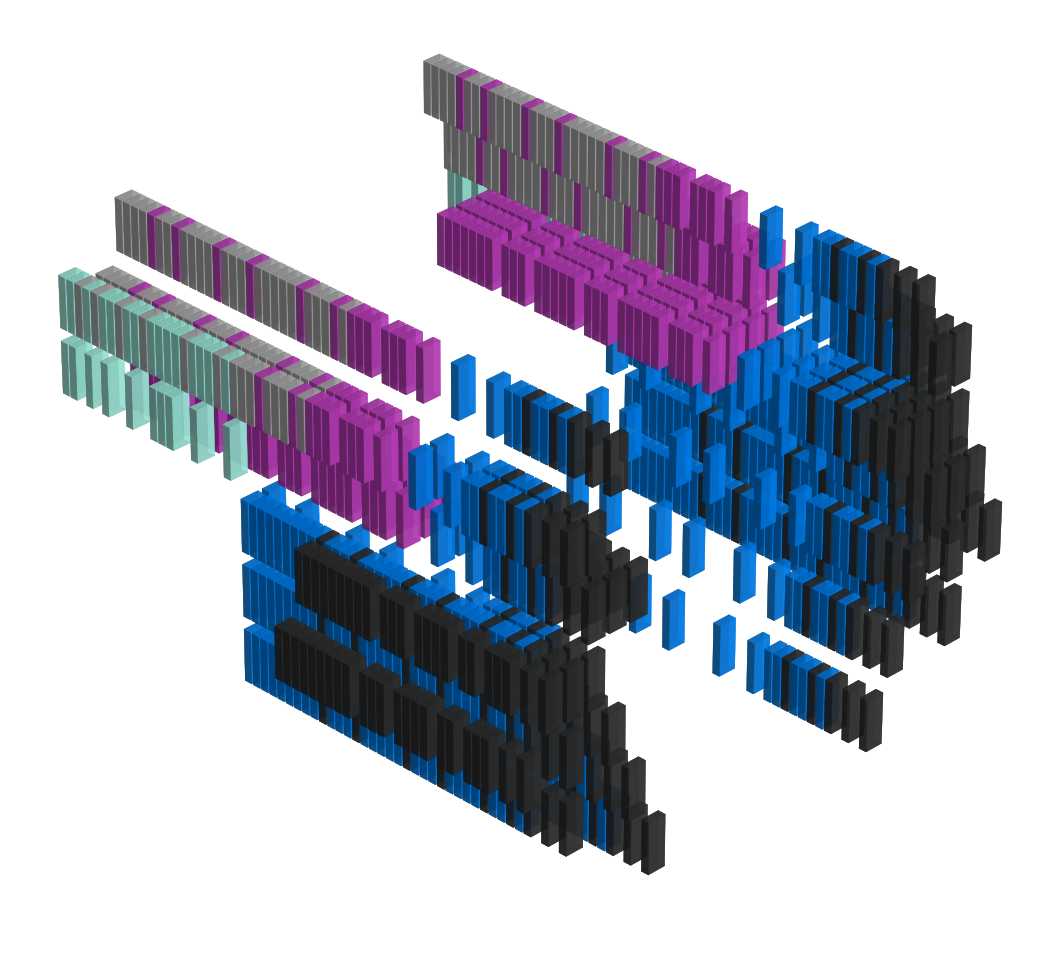
\includegraphics[width=14cm]{src/presets/pattern4-45.png}%           
    \end{adjustbox}                                                        
\caption{Evolution of Preset 4.}                                           
\end{figure}                                                               
\clearpage                                                                 
                                                                           
\begin{lstlisting}[basicstyle=\tiny,caption=Source code for Preset 4.]
preset4
        ; unusedPresetByte: Unused Byte
        .BYTE $00
        ; smoothingDelay: 'Because of the time taken to draw larger patterns speed
        ; increase/decrease is not linear. You can adjust the 'compensating delay'
        ; which often smooths out jerky patterns. Can be used just for special FX),
        ; though. Suck it and see.'
        .BYTE $0C
        ; cursorSpeed: 'Gives you a slow or fast little cursor, according to setting.'
        .BYTE $01
        ; bufferLength: 'Larger patterns flow more smoothly with a shorter
        ; Buffer Length - not so many positions are retained so less plotting to do.
        ; Small patterns with a long Buffer Length are good for 'steamer' effects.
        ; N.B. Cannot be adjusted whilst patterns are actually onscreen.'
        .BYTE $2B
        ; pulseSpeed: 'Usually if you hold down the button you get a continuous
        ; stream. Setting the Pulse Speed allows you to generate a pulsed stream, as
        ; if you were rapidly pressing and releasing the FIRE button.'
        .BYTE $01
        ; indexForColorBarDisplay: 'The initial index for the color displayed
        ; in the color bar when adjusting the colors for each step.'
        .BYTE $07
        ; lineWidth: 'Sets the width of the lines produced in Line Mode.'
        .BYTE $07
        ; sequencerSpeed: 'Controls the rate at which sequencer feeds in its data. '
        .BYTE $08
        ; pulseWidth: 'Sets the length of the pulses in a pulsed stream output.
        ; Don't worry about what that means - just get in there and mess with it.'
        .BYTE $01
        ; baseLevel: 'Controls how many 'levels' of pattern are plotted.'
        .BYTE $07
        ; presetColorValuesArray: 'Allows you to set the colour for each of the
        ; seven pattern steps. Set up the colour you want, press RETURN, and the
        ; command offers the next colour along, up to no. 7, then ends. Cannot be
        ; adjusted while patterns being generated.'
        .BYTE BLACK,GRAY1,BLUE,GRAY2,PURPLE,GRAY3,CYAN,WHITE
        ; trackingActivated: 'Controls whether logic-seeking is used in the
        ; buffer or not. The upshot of this for you is a slightly different feel -
        ; continuous but fragmented when ON, or together-ish bursts when OFF. Try it.'
        .BYTE $00
        ; lineModeActivated: 'A bit like drawing with the Aurora Borealis'
        .BYTE $00
        ; presetIndex: 'This calls in one of the 16 presets, stored Lightsynth
        ; parameters which give different effects. Try them all out io see some uf
        ; the multitude of effects which you cai achieve using the system. Some are
        ; fast, some slow, some pulse, others swirl. Play with them all, try them to
        ; different music.'
        .BYTE $01
        ; currentPatternElement: 'Initial pattern used by this preset.'
        .BYTE $01
        ; currentSymmetrySetting: 'Current symmetry setting.'
        ; Possible values are 0 - 4:
        ; 'NO SYMMETRY     '
        ; 'Y-AXIS SYMMETRY '
        ; 'X-Y SYMMETRY    '
        ; 'X-AXIS SYMMETRY '
        ; 'QUAD SYMMETRY   '
        .BYTE $01
        ; Unused Data.
        .BYTE $00,$FF,$00,$00,$FF,$00,$FF,$00,$FF
\end{lstlisting}


\clearpage                                                                 
\begin{figure}[H]                                                          
    \centering                                                             
    \begin{adjustbox}{width=14cm,center}                                   
      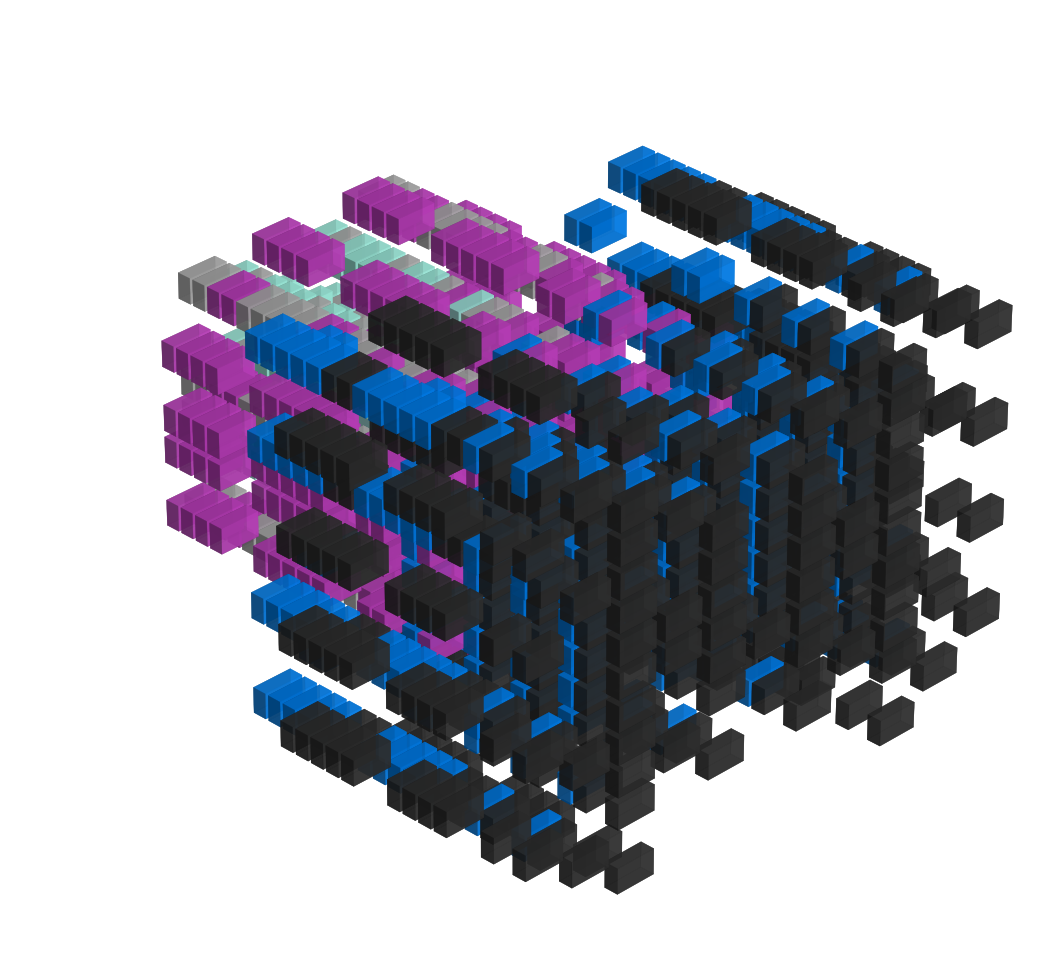
\includegraphics[width=14cm]{src/presets/pattern5-45.png}%           
    \end{adjustbox}                                                        
\caption{Evolution of Preset 5.}                                           
\end{figure}                                                               
\clearpage                                                                 
                                                                           
\begin{lstlisting}[basicstyle=\tiny,caption=Source code for Preset 5.]
preset5
        ; unusedPresetByte: Unused Byte
        .BYTE $00
        ; smoothingDelay: 'Because of the time taken to draw larger patterns speed
        ; increase/decrease is not linear. You can adjust the 'compensating delay'
        ; which often smooths out jerky patterns. Can be used just for special FX),
        ; though. Suck it and see.'
        .BYTE $0C
        ; cursorSpeed: 'Gives you a slow or fast little cursor, according to setting.'
        .BYTE $02
        ; bufferLength: 'Larger patterns flow more smoothly with a shorter
        ; Buffer Length - not so many positions are retained so less plotting to do.
        ; Small patterns with a long Buffer Length are good for 'steamer' effects.
        ; N.B. Cannot be adjusted whilst patterns are actually onscreen.'
        .BYTE $2B
        ; pulseSpeed: 'Usually if you hold down the button you get a continuous
        ; stream. Setting the Pulse Speed allows you to generate a pulsed stream, as
        ; if you were rapidly pressing and releasing the FIRE button.'
        .BYTE $01
        ; indexForColorBarDisplay: 'The initial index for the color displayed
        ; in the color bar when adjusting the colors for each step.'
        .BYTE $07
        ; lineWidth: 'Sets the width of the lines produced in Line Mode.'
        .BYTE $07
        ; sequencerSpeed: 'Controls the rate at which sequencer feeds in its data. '
        .BYTE $0C
        ; pulseWidth: 'Sets the length of the pulses in a pulsed stream output.
        ; Don't worry about what that means - just get in there and mess with it.'
        .BYTE $01
        ; baseLevel: 'Controls how many 'levels' of pattern are plotted.'
        .BYTE $07
        ; presetColorValuesArray: 'Allows you to set the colour for each of the
        ; seven pattern steps. Set up the colour you want, press RETURN, and the
        ; command offers the next colour along, up to no. 7, then ends. Cannot be
        ; adjusted while patterns being generated.'
        .BYTE BLACK,GRAY1,BLUE,GRAY2,PURPLE,GRAY3,CYAN,WHITE
        ; trackingActivated: 'Controls whether logic-seeking is used in the
        ; buffer or not. The upshot of this for you is a slightly different feel -
        ; continuous but fragmented when ON, or together-ish bursts when OFF. Try it.'
        .BYTE $00
        ; lineModeActivated: 'A bit like drawing with the Aurora Borealis'
        .BYTE $00
        ; presetIndex: 'This calls in one of the 16 presets, stored Lightsynth
        ; parameters which give different effects. Try them all out io see some uf
        ; the multitude of effects which you cai achieve using the system. Some are
        ; fast, some slow, some pulse, others swirl. Play with them all, try them to
        ; different music.'
        .BYTE $06
        ; currentPatternElement: 'Initial pattern used by this preset.'
        .BYTE $06
        ; currentSymmetrySetting: 'Current symmetry setting.'
        ; Possible values are 0 - 4:
        ; 'NO SYMMETRY     '
        ; 'Y-AXIS SYMMETRY '
        ; 'X-Y SYMMETRY    '
        ; 'X-AXIS SYMMETRY '
        ; 'QUAD SYMMETRY   '
        .BYTE $03
        ; Unused Data.
        .BYTE $00,$FF,$00,$00,$FF,$00,$FF,$00,$F7
\end{lstlisting}


\clearpage                                                                 
\begin{figure}[H]                                                          
    \centering                                                             
    \begin{adjustbox}{width=14cm,center}                                   
      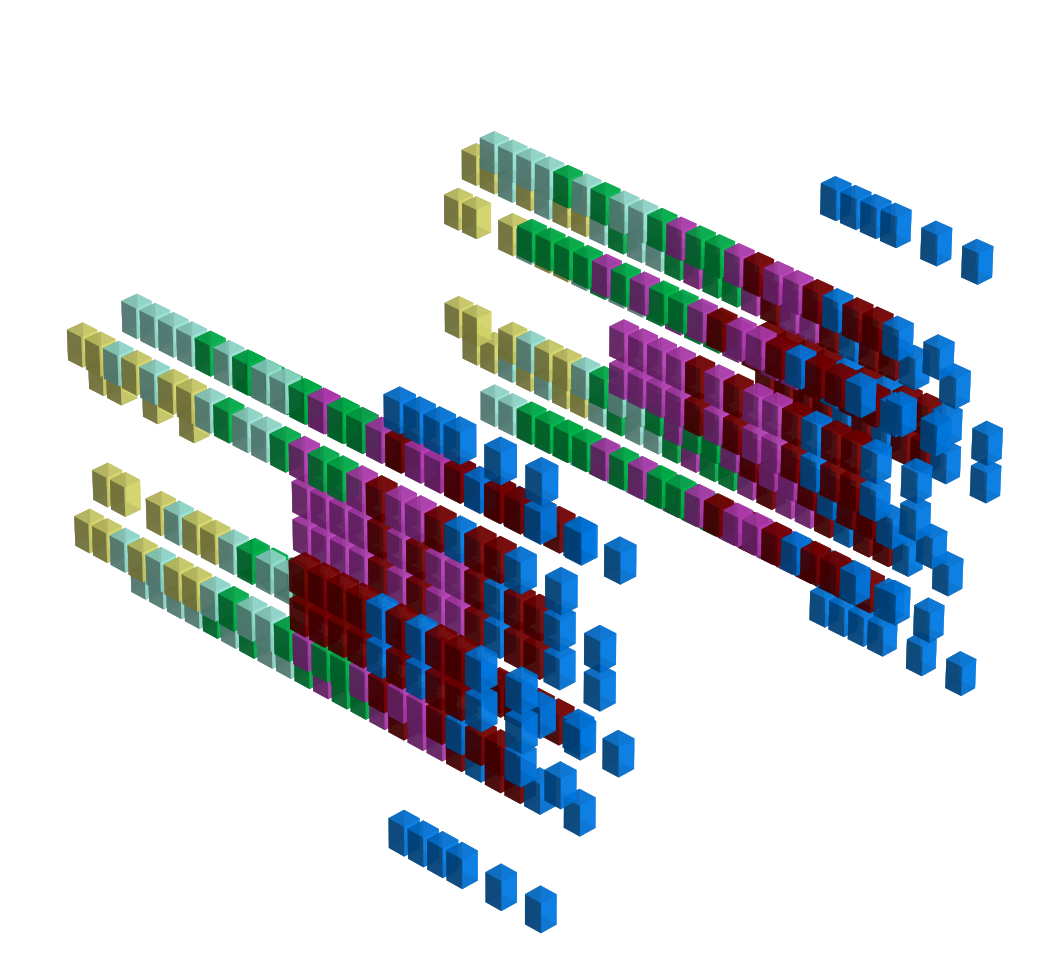
\includegraphics[width=14cm]{src/presets/pattern6-45.png}%           
    \end{adjustbox}                                                        
\caption{Evolution of Preset 6.}                                           
\end{figure}                                                               
\clearpage                                                                 
                                                                           
\begin{lstlisting}[basicstyle=\tiny,caption=Source code for Preset 6.]
preset6
        ; unusedPresetByte: Unused Byte
        .BYTE $00
        ; smoothingDelay: 'Because of the time taken to draw larger patterns speed
        ; increase/decrease is not linear. You can adjust the 'compensating delay'
        ; which often smooths out jerky patterns. Can be used just for special FX),
        ; though. Suck it and see.'
        .BYTE $0F
        ; cursorSpeed: 'Gives you a slow or fast little cursor, according to setting.'
        .BYTE $02
        ; bufferLength: 'Larger patterns flow more smoothly with a shorter
        ; Buffer Length - not so many positions are retained so less plotting to do.
        ; Small patterns with a long Buffer Length are good for 'steamer' effects.
        ; N.B. Cannot be adjusted whilst patterns are actually onscreen.'
        .BYTE $3F
        ; pulseSpeed: 'Usually if you hold down the button you get a continuous
        ; stream. Setting the Pulse Speed allows you to generate a pulsed stream, as
        ; if you were rapidly pressing and releasing the FIRE button.'
        .BYTE $01
        ; indexForColorBarDisplay: 'The initial index for the color displayed
        ; in the color bar when adjusting the colors for each step.'
        .BYTE $01
        ; lineWidth: 'Sets the width of the lines produced in Line Mode.'
        .BYTE $07
        ; sequencerSpeed: 'Controls the rate at which sequencer feeds in its data. '
        .BYTE $0F
        ; pulseWidth: 'Sets the length of the pulses in a pulsed stream output.
        ; Don't worry about what that means - just get in there and mess with it.'
        .BYTE $01
        ; baseLevel: 'Controls how many 'levels' of pattern are plotted.'
        .BYTE $07
        ; presetColorValuesArray: 'Allows you to set the colour for each of the
        ; seven pattern steps. Set up the colour you want, press RETURN, and the
        ; command offers the next colour along, up to no. 7, then ends. Cannot be
        ; adjusted while patterns being generated.'
        .BYTE BLACK,BLUE,RED,PURPLE,GREEN,CYAN,YELLOW,WHITE
        ; trackingActivated: 'Controls whether logic-seeking is used in the
        ; buffer or not. The upshot of this for you is a slightly different feel -
        ; continuous but fragmented when ON, or together-ish bursts when OFF. Try it.'
        .BYTE $FF
        ; lineModeActivated: 'A bit like drawing with the Aurora Borealis'
        .BYTE $00
        ; presetIndex: 'This calls in one of the 16 presets, stored Lightsynth
        ; parameters which give different effects. Try them all out io see some uf
        ; the multitude of effects which you cai achieve using the system. Some are
        ; fast, some slow, some pulse, others swirl. Play with them all, try them to
        ; different music.'
        .BYTE $03
        ; currentPatternElement: 'Initial pattern used by this preset.'
        .BYTE $03
        ; currentSymmetrySetting: 'Current symmetry setting.'
        ; Possible values are 0 - 4:
        ; 'NO SYMMETRY     '
        ; 'Y-AXIS SYMMETRY '
        ; 'X-Y SYMMETRY    '
        ; 'X-AXIS SYMMETRY '
        ; 'QUAD SYMMETRY   '
        .BYTE $04
        ; Unused Data.
        .BYTE $00,$FF,$00,$00,$FF,$00,$FF,$00,$FF
\end{lstlisting}


\clearpage                                                                 
\begin{figure}[H]                                                          
    \centering                                                             
    \begin{adjustbox}{width=14cm,center}                                   
      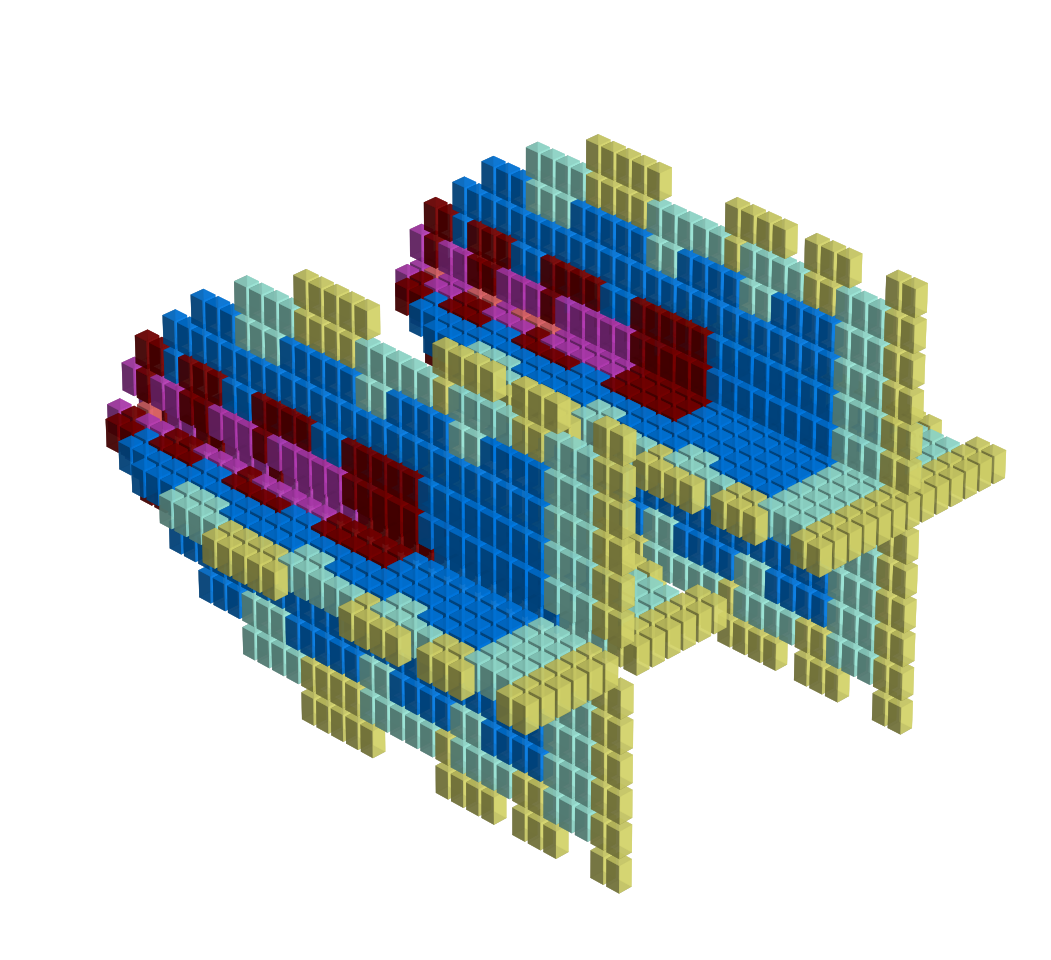
\includegraphics[width=14cm]{src/presets/pattern7-45.png}%           
    \end{adjustbox}                                                        
\caption{Evolution of Preset 7.}                                           
\end{figure}                                                               
\clearpage                                                                 
                                                                           
\begin{lstlisting}[basicstyle=\tiny,caption=Source code for Preset 7.]
preset7
        ; unusedPresetByte: Unused Byte
        .BYTE $00
        ; smoothingDelay: 'Because of the time taken to draw larger patterns speed
        ; increase/decrease is not linear. You can adjust the 'compensating delay'
        ; which often smooths out jerky patterns. Can be used just for special FX),
        ; though. Suck it and see.'
        .BYTE $0B
        ; cursorSpeed: 'Gives you a slow or fast little cursor, according to setting.'
        .BYTE $01
        ; bufferLength: 'Larger patterns flow more smoothly with a shorter
        ; Buffer Length - not so many positions are retained so less plotting to do.
        ; Small patterns with a long Buffer Length are good for 'steamer' effects.
        ; N.B. Cannot be adjusted whilst patterns are actually onscreen.'
        .BYTE $1C
        ; pulseSpeed: 'Usually if you hold down the button you get a continuous
        ; stream. Setting the Pulse Speed allows you to generate a pulsed stream, as
        ; if you were rapidly pressing and releasing the FIRE button.'
        .BYTE $02
        ; indexForColorBarDisplay: 'The initial index for the color displayed
        ; in the color bar when adjusting the colors for each step.'
        .BYTE $0A
        ; lineWidth: 'Sets the width of the lines produced in Line Mode.'
        .BYTE $07
        ; sequencerSpeed: 'Controls the rate at which sequencer feeds in its data. '
        .BYTE $09
        ; pulseWidth: 'Sets the length of the pulses in a pulsed stream output.
        ; Don't worry about what that means - just get in there and mess with it.'
        .BYTE $01
        ; baseLevel: 'Controls how many 'levels' of pattern are plotted.'
        .BYTE $07
        ; presetColorValuesArray: 'Allows you to set the colour for each of the
        ; seven pattern steps. Set up the colour you want, press RETURN, and the
        ; command offers the next colour along, up to no. 7, then ends. Cannot be
        ; adjusted while patterns being generated.'
        .BYTE BLACK,YELLOW,CYAN,LTBLUE,BLUE,RED,PURPLE,LTRED
        ; trackingActivated: 'Controls whether logic-seeking is used in the
        ; buffer or not. The upshot of this for you is a slightly different feel -
        ; continuous but fragmented when ON, or together-ish bursts when OFF. Try it.'
        .BYTE $00
        ; lineModeActivated: 'A bit like drawing with the Aurora Borealis'
        .BYTE $00
        ; presetIndex: 'This calls in one of the 16 presets, stored Lightsynth
        ; parameters which give different effects. Try them all out io see some uf
        ; the multitude of effects which you cai achieve using the system. Some are
        ; fast, some slow, some pulse, others swirl. Play with them all, try them to
        ; different music.'
        .BYTE $07
        ; currentPatternElement: 'Initial pattern used by this preset.'
        .BYTE $07
        ; currentSymmetrySetting: 'Current symmetry setting.'
        ; Possible values are 0 - 4:
        ; 'NO SYMMETRY     '
        ; 'Y-AXIS SYMMETRY '
        ; 'X-Y SYMMETRY    '
        ; 'X-AXIS SYMMETRY '
        ; 'QUAD SYMMETRY   '
        .BYTE $01
        ; Unused Data.
        .BYTE $00,$FF,$00,$00,$FF,$00,$FF,$15,$EF
\end{lstlisting}


\clearpage                                                                 
\begin{figure}[H]                                                          
    \centering                                                             
    \begin{adjustbox}{width=14cm,center}                                   
      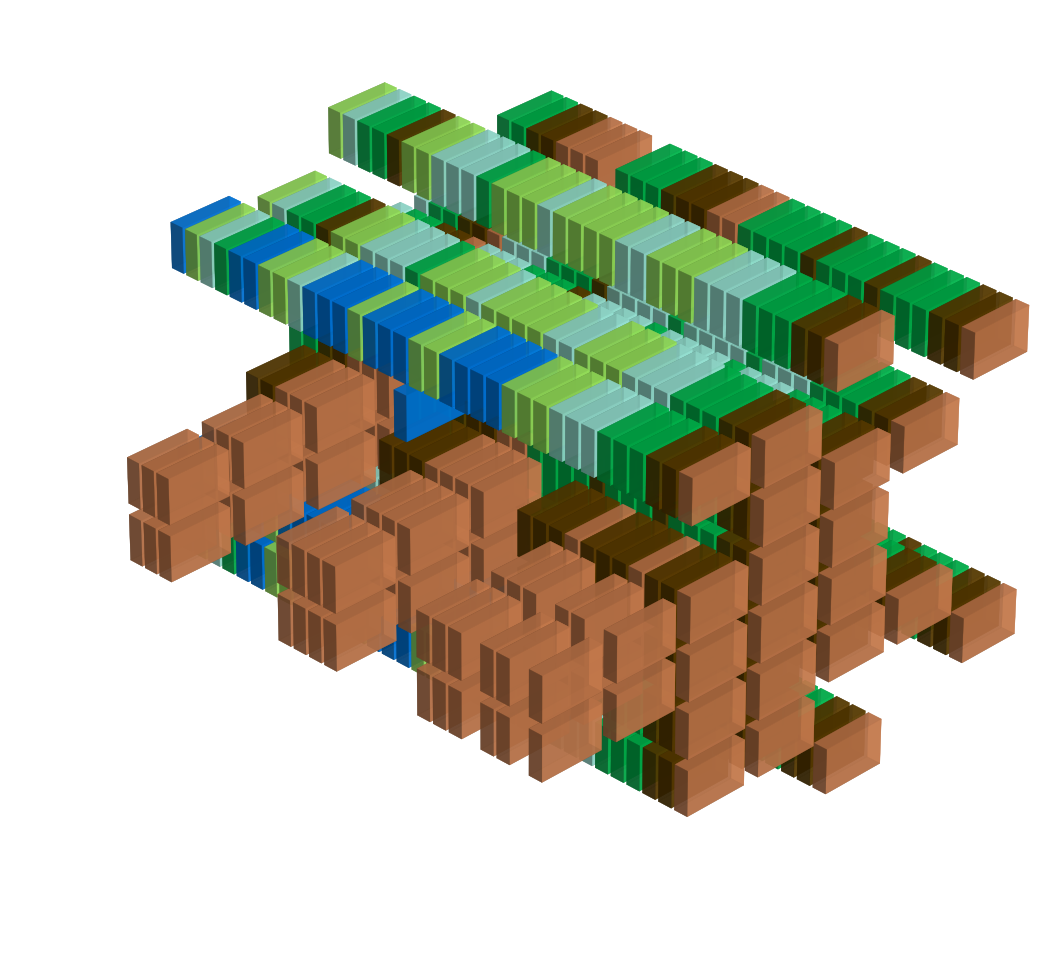
\includegraphics[width=14cm]{src/presets/pattern8-45.png}%           
    \end{adjustbox}                                                        
\caption{Evolution of Preset 8.}                                           
\end{figure}                                                               
\clearpage                                                                 
                                                                           
\begin{lstlisting}[basicstyle=\tiny,caption=Source code for Preset 8.]
preset8
        ; unusedPresetByte: Unused Byte
        .BYTE $00
        ; smoothingDelay: 'Because of the time taken to draw larger patterns speed
        ; increase/decrease is not linear. You can adjust the 'compensating delay'
        ; which often smooths out jerky patterns. Can be used just for special FX),
        ; though. Suck it and see.'
        .BYTE $04
        ; cursorSpeed: 'Gives you a slow or fast little cursor, according to setting.'
        .BYTE $01
        ; bufferLength: 'Larger patterns flow more smoothly with a shorter
        ; Buffer Length - not so many positions are retained so less plotting to do.
        ; Small patterns with a long Buffer Length are good for 'steamer' effects.
        ; N.B. Cannot be adjusted whilst patterns are actually onscreen.'
        .BYTE $28
        ; pulseSpeed: 'Usually if you hold down the button you get a continuous
        ; stream. Setting the Pulse Speed allows you to generate a pulsed stream, as
        ; if you were rapidly pressing and releasing the FIRE button.'
        .BYTE $02
        ; indexForColorBarDisplay: 'The initial index for the color displayed
        ; in the color bar when adjusting the colors for each step.'
        .BYTE $01
        ; lineWidth: 'Sets the width of the lines produced in Line Mode.'
        .BYTE $07
        ; sequencerSpeed: 'Controls the rate at which sequencer feeds in its data. '
        .BYTE $0A
        ; pulseWidth: 'Sets the length of the pulses in a pulsed stream output.
        ; Don't worry about what that means - just get in there and mess with it.'
        .BYTE $01
        ; baseLevel: 'Controls how many 'levels' of pattern are plotted.'
        .BYTE $07
        ; presetColorValuesArray: 'Allows you to set the colour for each of the
        ; seven pattern steps. Set up the colour you want, press RETURN, and the
        ; command offers the next colour along, up to no. 7, then ends. Cannot be
        ; adjusted while patterns being generated.'
        .BYTE BLACK,ORANGE,BROWN,GREEN,CYAN,LTGREEN,LTBLUE,BLUE
        ; trackingActivated: 'Controls whether logic-seeking is used in the
        ; buffer or not. The upshot of this for you is a slightly different feel -
        ; continuous but fragmented when ON, or together-ish bursts when OFF. Try it.'
        .BYTE $FF
        ; lineModeActivated: 'A bit like drawing with the Aurora Borealis'
        .BYTE $00
        ; presetIndex: 'This calls in one of the 16 presets, stored Lightsynth
        ; parameters which give different effects. Try them all out io see some uf
        ; the multitude of effects which you cai achieve using the system. Some are
        ; fast, some slow, some pulse, others swirl. Play with them all, try them to
        ; different music.'
        .BYTE $01
        ; currentPatternElement: 'Initial pattern used by this preset.'
        .BYTE $01
        ; currentSymmetrySetting: 'Current symmetry setting.'
        ; Possible values are 0 - 4:
        ; 'NO SYMMETRY     '
        ; 'Y-AXIS SYMMETRY '
        ; 'X-Y SYMMETRY    '
        ; 'X-AXIS SYMMETRY '
        ; 'QUAD SYMMETRY   '
        .BYTE $03
        ; Unused Data.
        .BYTE $FF,$00,$FF,$FF,$00,$FF,$00,$FF,$00
\end{lstlisting}


\clearpage                                                                 
\begin{figure}[H]                                                          
    \centering                                                             
    \begin{adjustbox}{width=14cm,center}                                   
      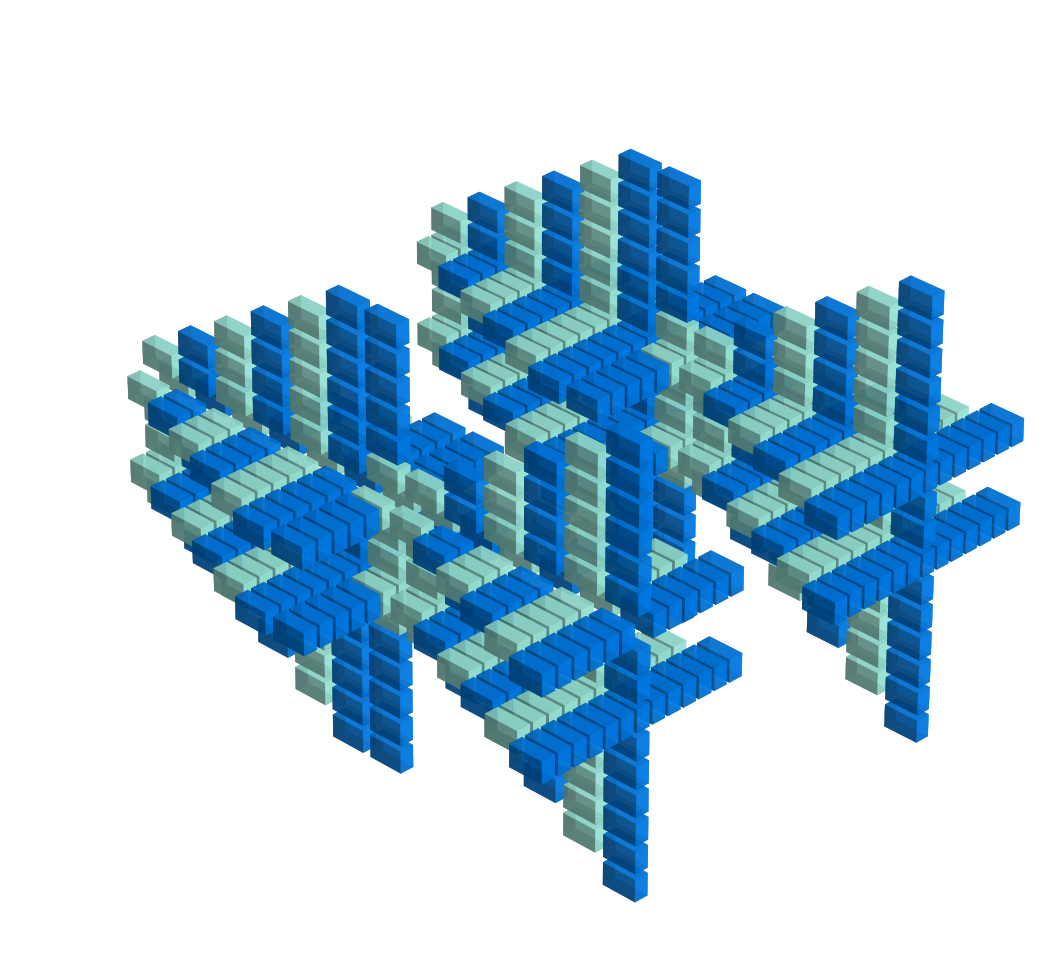
\includegraphics[width=14cm]{src/presets/pattern9-45.png}%           
    \end{adjustbox}                                                        
\caption{Evolution of Preset 9.}                                           
\end{figure}                                                               
\clearpage                                                                 
                                                                           
\begin{lstlisting}[basicstyle=\tiny,caption=Source code for Preset 9.]
preset9
        ; unusedPresetByte: Unused Byte
        .BYTE $00
        ; smoothingDelay: 'Because of the time taken to draw larger patterns speed
        ; increase/decrease is not linear. You can adjust the 'compensating delay'
        ; which often smooths out jerky patterns. Can be used just for special FX),
        ; though. Suck it and see.'
        .BYTE $11
        ; cursorSpeed: 'Gives you a slow or fast little cursor, according to setting.'
        .BYTE $01
        ; bufferLength: 'Larger patterns flow more smoothly with a shorter
        ; Buffer Length - not so many positions are retained so less plotting to do.
        ; Small patterns with a long Buffer Length are good for 'steamer' effects.
        ; N.B. Cannot be adjusted whilst patterns are actually onscreen.'
        .BYTE $0D
        ; pulseSpeed: 'Usually if you hold down the button you get a continuous
        ; stream. Setting the Pulse Speed allows you to generate a pulsed stream, as
        ; if you were rapidly pressing and releasing the FIRE button.'
        .BYTE $07
        ; indexForColorBarDisplay: 'The initial index for the color displayed
        ; in the color bar when adjusting the colors for each step.'
        .BYTE $01
        ; lineWidth: 'Sets the width of the lines produced in Line Mode.'
        .BYTE $07
        ; sequencerSpeed: 'Controls the rate at which sequencer feeds in its data. '
        .BYTE $0C
        ; pulseWidth: 'Sets the length of the pulses in a pulsed stream output.
        ; Don't worry about what that means - just get in there and mess with it.'
        .BYTE $01
        ; baseLevel: 'Controls how many 'levels' of pattern are plotted.'
        .BYTE $07
        ; presetColorValuesArray: 'Allows you to set the colour for each of the
        ; seven pattern steps. Set up the colour you want, press RETURN, and the
        ; command offers the next colour along, up to no. 7, then ends. Cannot be
        ; adjusted while patterns being generated.'
        .BYTE BLACK,BLUE,CYAN,BLUE,CYAN,BLUE,CYAN,BLUE
        ; trackingActivated: 'Controls whether logic-seeking is used in the
        ; buffer or not. The upshot of this for you is a slightly different feel -
        ; continuous but fragmented when ON, or together-ish bursts when OFF. Try it.'
        .BYTE $FF
        ; lineModeActivated: 'A bit like drawing with the Aurora Borealis'
        .BYTE $00
        ; presetIndex: 'This calls in one of the 16 presets, stored Lightsynth
        ; parameters which give different effects. Try them all out io see some uf
        ; the multitude of effects which you cai achieve using the system. Some are
        ; fast, some slow, some pulse, others swirl. Play with them all, try them to
        ; different music.'
        .BYTE $07
        ; currentPatternElement: 'Initial pattern used by this preset.'
        .BYTE $07
        ; currentSymmetrySetting: 'Current symmetry setting.'
        ; Possible values are 0 - 4:
        ; 'NO SYMMETRY     '
        ; 'Y-AXIS SYMMETRY '
        ; 'X-Y SYMMETRY    '
        ; 'X-AXIS SYMMETRY '
        ; 'QUAD SYMMETRY   '
        .BYTE $04
        ; Unused Data.
        .BYTE $FF,$00,$FF,$FF,$00,$FF,$00,$FF,$00
\end{lstlisting}


\clearpage                                                                 
\begin{figure}[H]                                                          
    \centering                                                             
    \begin{adjustbox}{width=14cm,center}                                   
      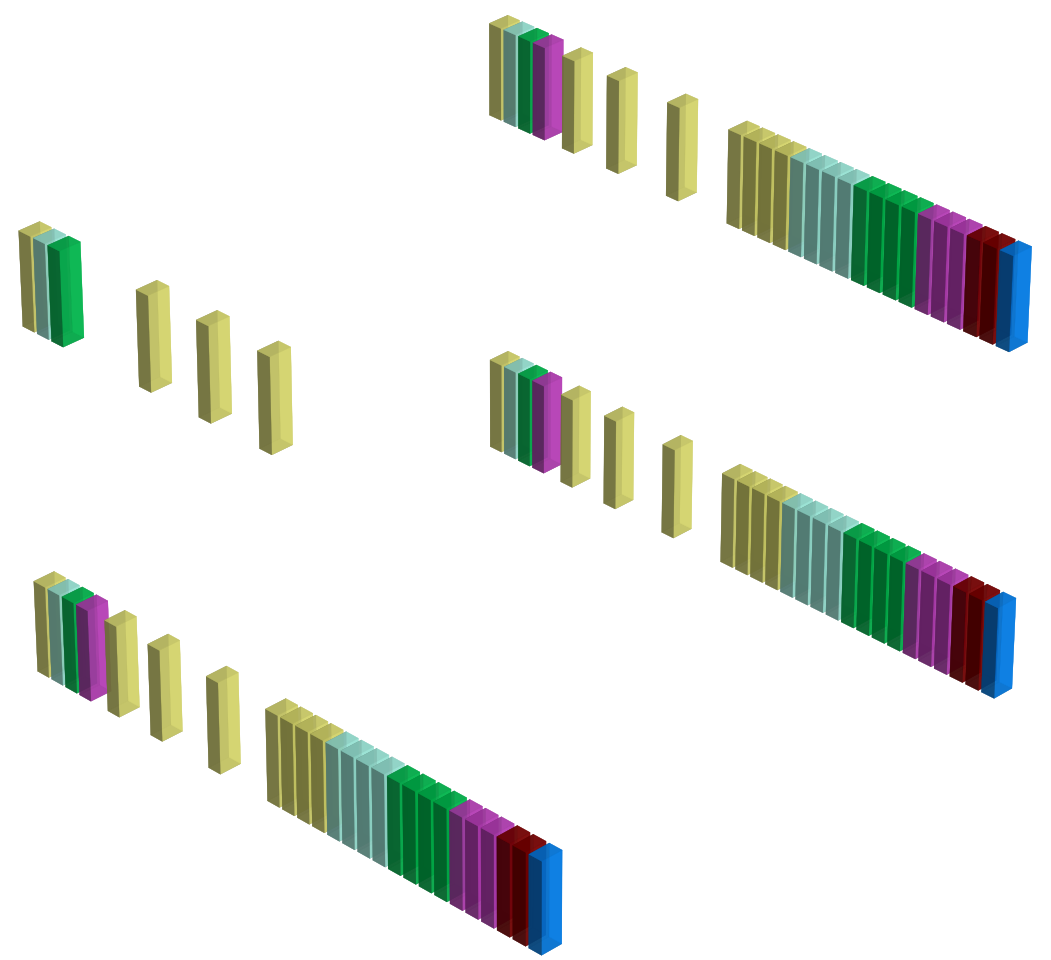
\includegraphics[width=14cm]{src/presets/pattern10-45.png}%           
    \end{adjustbox}                                                        
\caption{Evolution of Preset 10.}                                           
\end{figure}                                                               
\clearpage                                                                 
                                                                           
\begin{lstlisting}[basicstyle=\tiny,caption=Source code for Preset 10.]
preset10
        ; unusedPresetByte: Unused Byte
        .BYTE $00
        ; smoothingDelay: 'Because of the time taken to draw larger patterns speed
        ; increase/decrease is not linear. You can adjust the 'compensating delay'
        ; which often smooths out jerky patterns. Can be used just for special FX),
        ; though. Suck it and see.'
        .BYTE $01
        ; cursorSpeed: 'Gives you a slow or fast little cursor, according to setting.'
        .BYTE $02
        ; bufferLength: 'Larger patterns flow more smoothly with a shorter
        ; Buffer Length - not so many positions are retained so less plotting to do.
        ; Small patterns with a long Buffer Length are good for 'steamer' effects.
        ; N.B. Cannot be adjusted whilst patterns are actually onscreen.'
        .BYTE $1F
        ; pulseSpeed: 'Usually if you hold down the button you get a continuous
        ; stream. Setting the Pulse Speed allows you to generate a pulsed stream, as
        ; if you were rapidly pressing and releasing the FIRE button.'
        .BYTE $02
        ; indexForColorBarDisplay: 'The initial index for the color displayed
        ; in the color bar when adjusting the colors for each step.'
        .BYTE $09
        ; lineWidth: 'Sets the width of the lines produced in Line Mode.'
        .BYTE $04
        ; sequencerSpeed: 'Controls the rate at which sequencer feeds in its data. '
        .BYTE $08
        ; pulseWidth: 'Sets the length of the pulses in a pulsed stream output.
        ; Don't worry about what that means - just get in there and mess with it.'
        .BYTE $01
        ; baseLevel: 'Controls how many 'levels' of pattern are plotted.'
        .BYTE $07
        ; presetColorValuesArray: 'Allows you to set the colour for each of the
        ; seven pattern steps. Set up the colour you want, press RETURN, and the
        ; command offers the next colour along, up to no. 7, then ends. Cannot be
        ; adjusted while patterns being generated.'
        .BYTE BLACK,BLUE,RED,RED,PURPLE,LTRED,ORANGE,BROWN
        ; trackingActivated: 'Controls whether logic-seeking is used in the
        ; buffer or not. The upshot of this for you is a slightly different feel -
        ; continuous but fragmented when ON, or together-ish bursts when OFF. Try it.'
        .BYTE $FF
        ; lineModeActivated: 'A bit like drawing with the Aurora Borealis'
        .BYTE $01
        ; presetIndex: 'This calls in one of the 16 presets, stored Lightsynth
        ; parameters which give different effects. Try them all out io see some uf
        ; the multitude of effects which you cai achieve using the system. Some are
        ; fast, some slow, some pulse, others swirl. Play with them all, try them to
        ; different music.'
        .BYTE $00
        ; currentPatternElement: 'Initial pattern used by this preset.'
        .BYTE $00
        ; currentSymmetrySetting: 'Current symmetry setting.'
        ; Possible values are 0 - 4:
        ; 'NO SYMMETRY     '
        ; 'Y-AXIS SYMMETRY '
        ; 'X-Y SYMMETRY    '
        ; 'X-AXIS SYMMETRY '
        ; 'QUAD SYMMETRY   '
        .BYTE $04
        ; Unused Data.
        .BYTE $FF,$00,$FF,$FF,$00,$FF,$00,$FF,$00
\end{lstlisting}


\clearpage                                                                 
\begin{figure}[H]                                                          
    \centering                                                             
    \begin{adjustbox}{width=14cm,center}                                   
      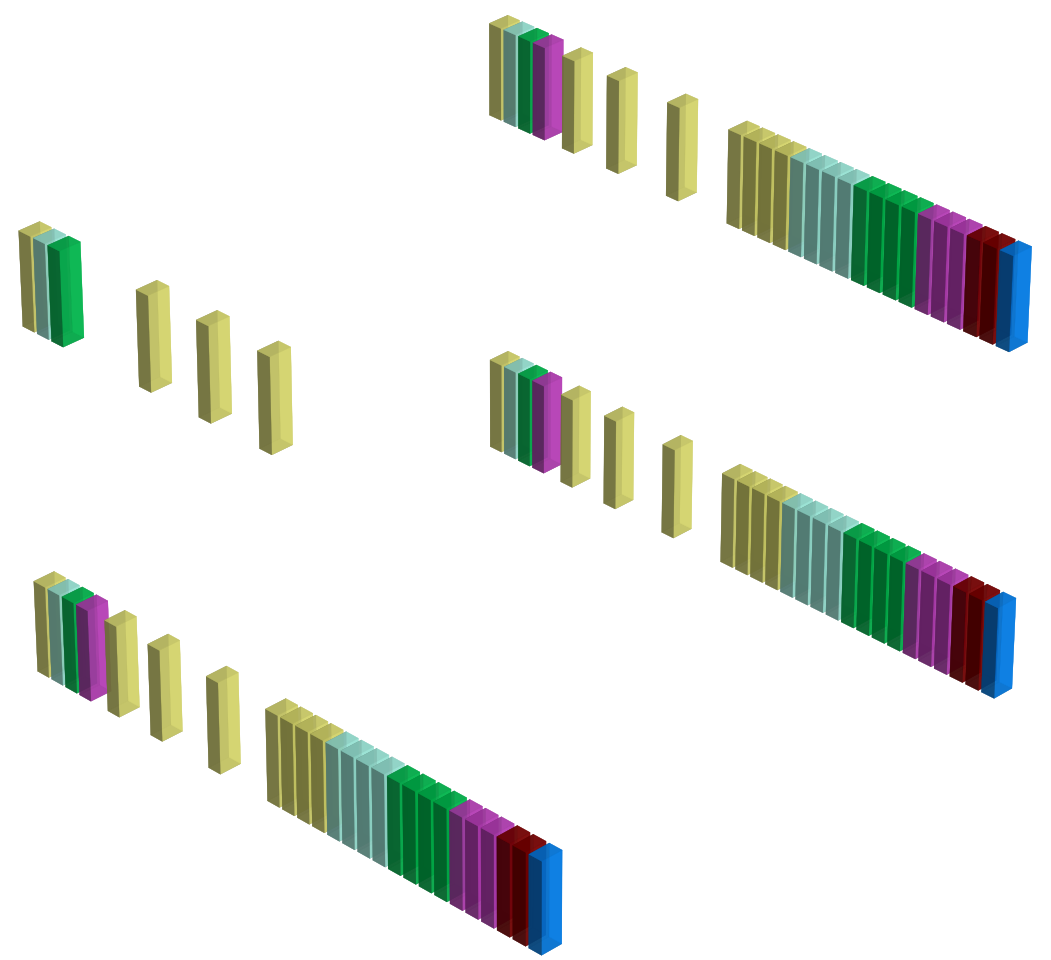
\includegraphics[width=14cm]{src/presets/pattern10-45.png}%           
    \end{adjustbox}                                                        
\caption{Evolution of Preset 11.}                                           
\end{figure}                                                               
\clearpage                                                                 
                                                                           
\begin{lstlisting}[basicstyle=\tiny,caption=Source code for Preset 11.]
preset11
        ; unusedPresetByte: Unused Byte
        .BYTE $00
        ; smoothingDelay: 'Because of the time taken to draw larger patterns speed
        ; increase/decrease is not linear. You can adjust the 'compensating delay'
        ; which often smooths out jerky patterns. Can be used just for special FX),
        ; though. Suck it and see.'
        .BYTE $01
        ; cursorSpeed: 'Gives you a slow or fast little cursor, according to setting.'
        .BYTE $01
        ; bufferLength: 'Larger patterns flow more smoothly with a shorter
        ; Buffer Length - not so many positions are retained so less plotting to do.
        ; Small patterns with a long Buffer Length are good for 'steamer' effects.
        ; N.B. Cannot be adjusted whilst patterns are actually onscreen.'
        .BYTE $13
        ; pulseSpeed: 'Usually if you hold down the button you get a continuous
        ; stream. Setting the Pulse Speed allows you to generate a pulsed stream, as
        ; if you were rapidly pressing and releasing the FIRE button.'
        .BYTE $06
        ; indexForColorBarDisplay: 'The initial index for the color displayed
        ; in the color bar when adjusting the colors for each step.'
        .BYTE $01
        ; lineWidth: 'Sets the width of the lines produced in Line Mode.'
        .BYTE $07
        ; sequencerSpeed: 'Controls the rate at which sequencer feeds in its data. '
        .BYTE $08
        ; pulseWidth: 'Sets the length of the pulses in a pulsed stream output.
        ; Don't worry about what that means - just get in there and mess with it.'
        .BYTE $05
        ; baseLevel: 'Controls how many 'levels' of pattern are plotted.'
        .BYTE $07
        ; presetColorValuesArray: 'Allows you to set the colour for each of the
        ; seven pattern steps. Set up the colour you want, press RETURN, and the
        ; command offers the next colour along, up to no. 7, then ends. Cannot be
        ; adjusted while patterns being generated.'
        .BYTE BLACK,BLUE,RED,PURPLE,GREEN,CYAN,YELLOW,WHITE
        ; trackingActivated: 'Controls whether logic-seeking is used in the
        ; buffer or not. The upshot of this for you is a slightly different feel -
        ; continuous but fragmented when ON, or together-ish bursts when OFF. Try it.'
        .BYTE $FF
        ; lineModeActivated: 'A bit like drawing with the Aurora Borealis'
        .BYTE $00
        ; presetIndex: 'This calls in one of the 16 presets, stored Lightsynth
        ; parameters which give different effects. Try them all out io see some uf
        ; the multitude of effects which you cai achieve using the system. Some are
        ; fast, some slow, some pulse, others swirl. Play with them all, try them to
        ; different music.'
        .BYTE $0F
        ; currentPatternElement: 'Initial pattern used by this preset.'
        .BYTE $0F
        ; currentSymmetrySetting: 'Current symmetry setting.'
        ; Possible values are 0 - 4:
        ; 'NO SYMMETRY     '
        ; 'Y-AXIS SYMMETRY '
        ; 'X-Y SYMMETRY    '
        ; 'X-AXIS SYMMETRY '
        ; 'QUAD SYMMETRY   '
        .BYTE $04
        ; Unused Data.
        .BYTE $FF,$00,$FF,$FF,$00,$FF,$00,$EA,$10
\end{lstlisting}


\clearpage                                                                 
\begin{figure}[H]                                                          
    \centering                                                             
    \begin{adjustbox}{width=14cm,center}                                   
      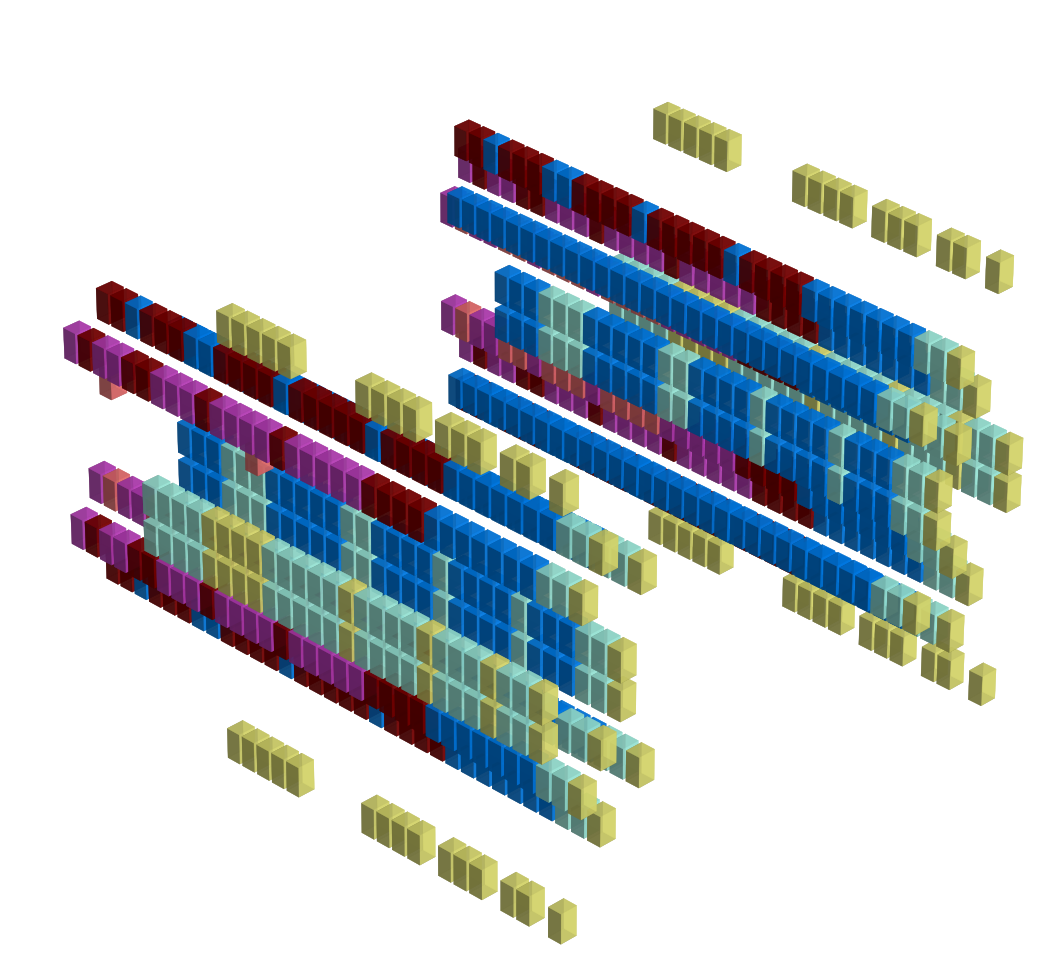
\includegraphics[width=14cm]{src/presets/pattern12-45.png}%           
    \end{adjustbox}                                                        
\caption{Evolution of Preset 12.}                                           
\end{figure}                                                               
\clearpage                                                                 
                                                                           
\begin{lstlisting}[basicstyle=\tiny,caption=Source code for Preset 12.]
preset12
        ; unusedPresetByte: Unused Byte
        .BYTE $00
        ; smoothingDelay: 'Because of the time taken to draw larger patterns speed
        ; increase/decrease is not linear. You can adjust the 'compensating delay'
        ; which often smooths out jerky patterns. Can be used just for special FX),
        ; though. Suck it and see.'
        .BYTE $0C
        ; cursorSpeed: 'Gives you a slow or fast little cursor, according to setting.'
        .BYTE $02
        ; bufferLength: 'Larger patterns flow more smoothly with a shorter
        ; Buffer Length - not so many positions are retained so less plotting to do.
        ; Small patterns with a long Buffer Length are good for 'steamer' effects.
        ; N.B. Cannot be adjusted whilst patterns are actually onscreen.'
        .BYTE $28
        ; pulseSpeed: 'Usually if you hold down the button you get a continuous
        ; stream. Setting the Pulse Speed allows you to generate a pulsed stream, as
        ; if you were rapidly pressing and releasing the FIRE button.'
        .BYTE $01
        ; indexForColorBarDisplay: 'The initial index for the color displayed
        ; in the color bar when adjusting the colors for each step.'
        .BYTE $02
        ; lineWidth: 'Sets the width of the lines produced in Line Mode.'
        .BYTE $07
        ; sequencerSpeed: 'Controls the rate at which sequencer feeds in its data. '
        .BYTE $09
        ; pulseWidth: 'Sets the length of the pulses in a pulsed stream output.
        ; Don't worry about what that means - just get in there and mess with it.'
        .BYTE $01
        ; baseLevel: 'Controls how many 'levels' of pattern are plotted.'
        .BYTE $07
        ; presetColorValuesArray: 'Allows you to set the colour for each of the
        ; seven pattern steps. Set up the colour you want, press RETURN, and the
        ; command offers the next colour along, up to no. 7, then ends. Cannot be
        ; adjusted while patterns being generated.'
        .BYTE BLACK,BLUE,LTBLUE,CYAN,LTGREEN,YELLOW,PURPLE,RED
        ; trackingActivated: 'Controls whether logic-seeking is used in the
        ; buffer or not. The upshot of this for you is a slightly different feel -
        ; continuous but fragmented when ON, or together-ish bursts when OFF. Try it.'
        .BYTE $00
        ; lineModeActivated: 'A bit like drawing with the Aurora Borealis'
        .BYTE $00
        ; presetIndex: 'This calls in one of the 16 presets, stored Lightsynth
        ; parameters which give different effects. Try them all out io see some uf
        ; the multitude of effects which you cai achieve using the system. Some are
        ; fast, some slow, some pulse, others swirl. Play with them all, try them to
        ; different music.'
        .BYTE $0A
        ; currentPatternElement: 'Initial pattern used by this preset.'
        .BYTE $0A
        ; currentSymmetrySetting: 'Current symmetry setting.'
        ; Possible values are 0 - 4:
        ; 'NO SYMMETRY     '
        ; 'Y-AXIS SYMMETRY '
        ; 'X-Y SYMMETRY    '
        ; 'X-AXIS SYMMETRY '
        ; 'QUAD SYMMETRY   '
        .BYTE $01
        ; Unused Data.
        .BYTE $00,$FF,$00,$00,$FF,$00,$FF,$00,$FF
\end{lstlisting}


\clearpage                                                                 
\begin{figure}[H]                                                          
    \centering                                                             
    \begin{adjustbox}{width=14cm,center}                                   
      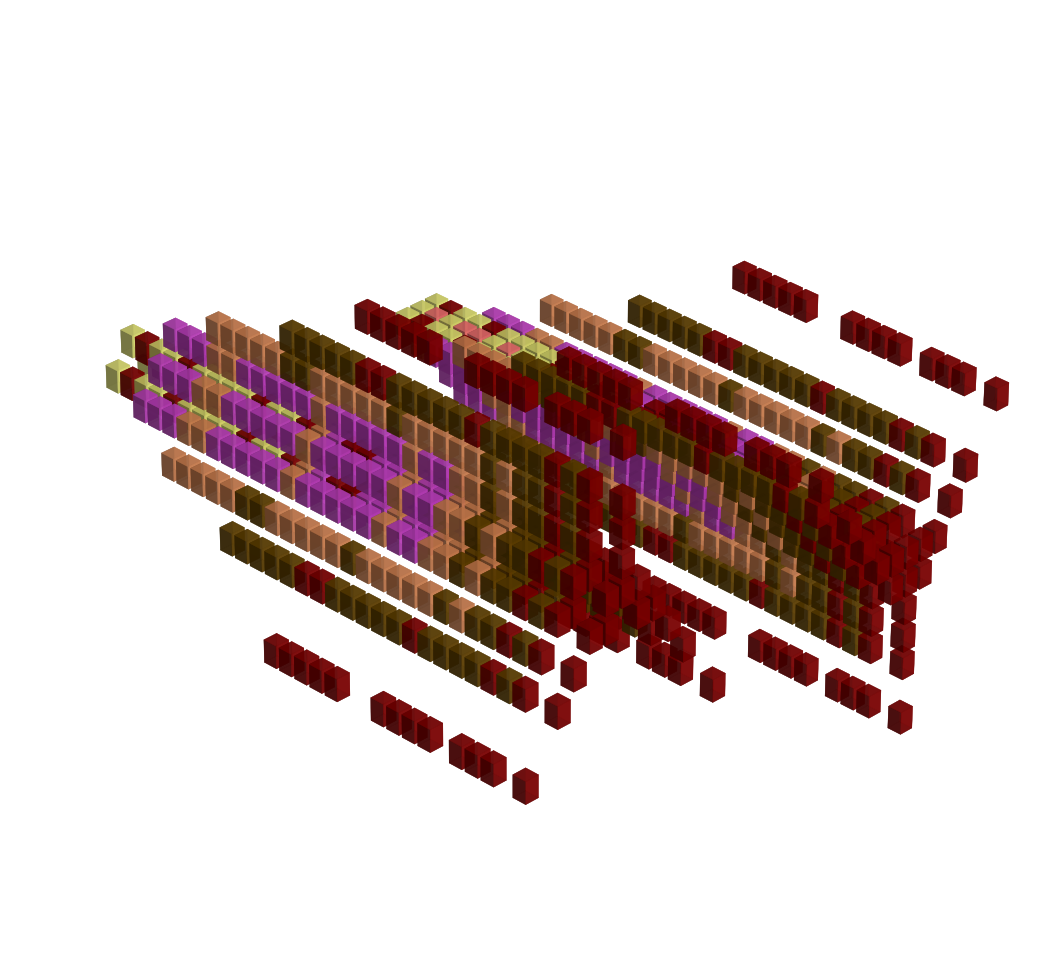
\includegraphics[width=14cm]{src/presets/pattern13-45.png}%           
    \end{adjustbox}                                                        
\caption{Evolution of Preset 13.}                                           
\end{figure}                                                               
\clearpage                                                                 
                                                                           
\begin{lstlisting}[basicstyle=\tiny,caption=Source code for Preset 13.]
preset13
        ; unusedPresetByte: Unused Byte
        .BYTE $00
        ; smoothingDelay: 'Because of the time taken to draw larger patterns speed
        ; increase/decrease is not linear. You can adjust the 'compensating delay'
        ; which often smooths out jerky patterns. Can be used just for special FX),
        ; though. Suck it and see.'
        .BYTE $0B
        ; cursorSpeed: 'Gives you a slow or fast little cursor, according to setting.'
        .BYTE $01
        ; bufferLength: 'Larger patterns flow more smoothly with a shorter
        ; Buffer Length - not so many positions are retained so less plotting to do.
        ; Small patterns with a long Buffer Length are good for 'steamer' effects.
        ; N.B. Cannot be adjusted whilst patterns are actually onscreen.'
        .BYTE $1C
        ; pulseSpeed: 'Usually if you hold down the button you get a continuous
        ; stream. Setting the Pulse Speed allows you to generate a pulsed stream, as
        ; if you were rapidly pressing and releasing the FIRE button.'
        .BYTE $02
        ; indexForColorBarDisplay: 'The initial index for the color displayed
        ; in the color bar when adjusting the colors for each step.'
        .BYTE $0A
        ; lineWidth: 'Sets the width of the lines produced in Line Mode.'
        .BYTE $07
        ; sequencerSpeed: 'Controls the rate at which sequencer feeds in its data. '
        .BYTE $09
        ; pulseWidth: 'Sets the length of the pulses in a pulsed stream output.
        ; Don't worry about what that means - just get in there and mess with it.'
        .BYTE $01
        ; baseLevel: 'Controls how many 'levels' of pattern are plotted.'
        .BYTE $07
        ; presetColorValuesArray: 'Allows you to set the colour for each of the
        ; seven pattern steps. Set up the colour you want, press RETURN, and the
        ; command offers the next colour along, up to no. 7, then ends. Cannot be
        ; adjusted while patterns being generated.'
        .BYTE BLACK,YELLOW,CYAN,LTBLUE,BLUE,RED,PURPLE,LTRED
        ; trackingActivated: 'Controls whether logic-seeking is used in the
        ; buffer or not. The upshot of this for you is a slightly different feel -
        ; continuous but fragmented when ON, or together-ish bursts when OFF. Try it.'
        .BYTE $00
        ; lineModeActivated: 'A bit like drawing with the Aurora Borealis'
        .BYTE $00
        ; presetIndex: 'This calls in one of the 16 presets, stored Lightsynth
        ; parameters which give different effects. Try them all out io see some uf
        ; the multitude of effects which you cai achieve using the system. Some are
        ; fast, some slow, some pulse, others swirl. Play with them all, try them to
        ; different music.'
        .BYTE $03
        ; currentPatternElement: 'Initial pattern used by this preset.'
        .BYTE $03
        ; currentSymmetrySetting: 'Current symmetry setting.'
        ; Possible values are 0 - 4:
        ; 'NO SYMMETRY     '
        ; 'Y-AXIS SYMMETRY '
        ; 'X-Y SYMMETRY    '
        ; 'X-AXIS SYMMETRY '
        ; 'QUAD SYMMETRY   '
        .BYTE $04
        ; Unused Data.
        .BYTE $00,$FF,$00,$00,$FF,$00,$FF,$00,$FF
\end{lstlisting}


\clearpage                                                                 
\begin{figure}[H]                                                          
    \centering                                                             
    \begin{adjustbox}{width=14cm,center}                                   
      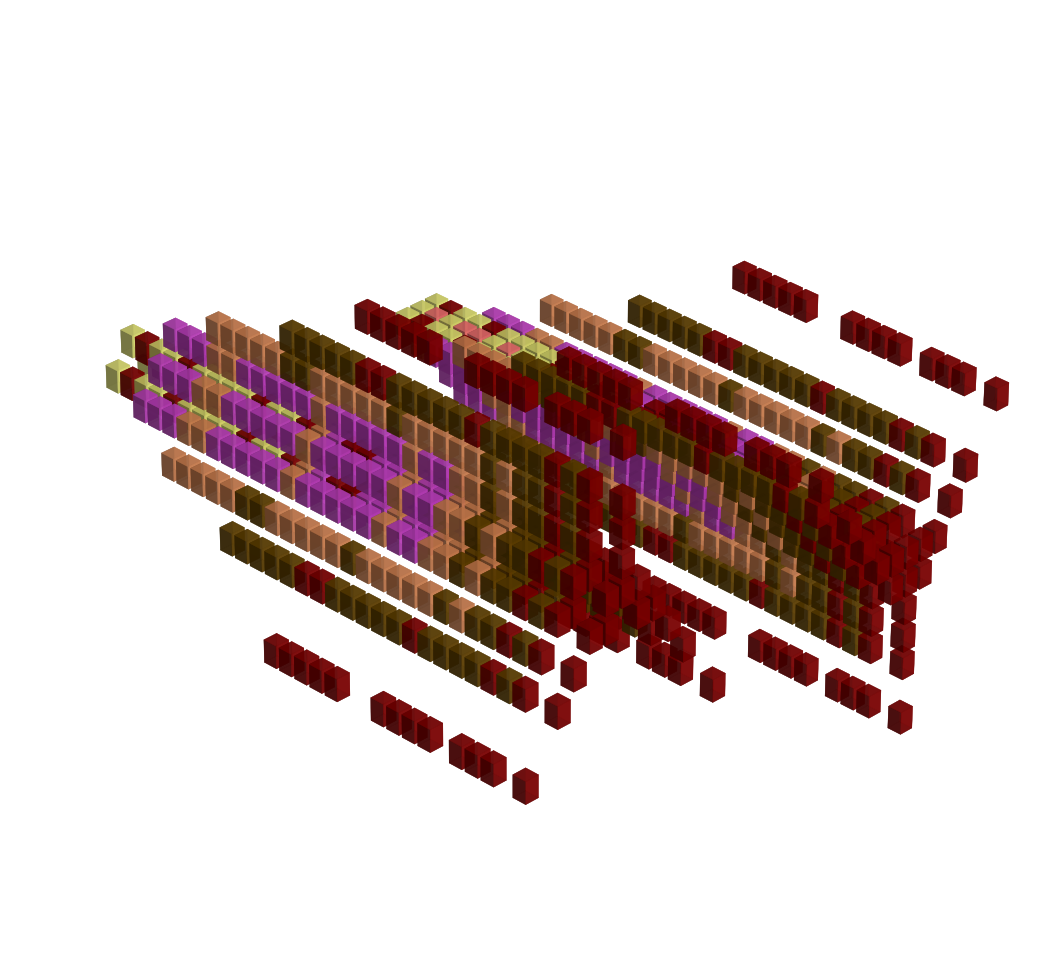
\includegraphics[width=14cm]{src/presets/pattern14-45.png}%           
    \end{adjustbox}                                                        
\caption{Evolution of Preset 14.}                                           
\end{figure}                                                               
\clearpage                                                                 
                                                                           
\begin{lstlisting}[basicstyle=\tiny,caption=Source code for Preset 14.]
preset14
        ; unusedPresetByte: Unused Byte
        .BYTE $00
        ; smoothingDelay: 'Because of the time taken to draw larger patterns speed
        ; increase/decrease is not linear. You can adjust the 'compensating delay'
        ; which often smooths out jerky patterns. Can be used just for special FX),
        ; though. Suck it and see.'
        .BYTE $0C
        ; cursorSpeed: 'Gives you a slow or fast little cursor, according to setting.'
        .BYTE $02
        ; bufferLength: 'Larger patterns flow more smoothly with a shorter
        ; Buffer Length - not so many positions are retained so less plotting to do.
        ; Small patterns with a long Buffer Length are good for 'steamer' effects.
        ; N.B. Cannot be adjusted whilst patterns are actually onscreen.'
        .BYTE $2B
        ; pulseSpeed: 'Usually if you hold down the button you get a continuous
        ; stream. Setting the Pulse Speed allows you to generate a pulsed stream, as
        ; if you were rapidly pressing and releasing the FIRE button.'
        .BYTE $01
        ; indexForColorBarDisplay: 'The initial index for the color displayed
        ; in the color bar when adjusting the colors for each step.'
        .BYTE $0A
        ; lineWidth: 'Sets the width of the lines produced in Line Mode.'
        .BYTE $07
        ; sequencerSpeed: 'Controls the rate at which sequencer feeds in its data. '
        .BYTE $08
        ; pulseWidth: 'Sets the length of the pulses in a pulsed stream output.
        ; Don't worry about what that means - just get in there and mess with it.'
        .BYTE $01
        ; baseLevel: 'Controls how many 'levels' of pattern are plotted.'
        .BYTE $07
        ; presetColorValuesArray: 'Allows you to set the colour for each of the
        ; seven pattern steps. Set up the colour you want, press RETURN, and the
        ; command offers the next colour along, up to no. 7, then ends. Cannot be
        ; adjusted while patterns being generated.'
        .BYTE BLACK,RED,BROWN,ORANGE,PURPLE,RED,YELLOW,LTRED
        ; trackingActivated: 'Controls whether logic-seeking is used in the
        ; buffer or not. The upshot of this for you is a slightly different feel -
        ; continuous but fragmented when ON, or together-ish bursts when OFF. Try it.'
        .BYTE $FF
        ; lineModeActivated: 'A bit like drawing with the Aurora Borealis'
        .BYTE $00
        ; presetIndex: 'This calls in one of the 16 presets, stored Lightsynth
        ; parameters which give different effects. Try them all out io see some uf
        ; the multitude of effects which you cai achieve using the system. Some are
        ; fast, some slow, some pulse, others swirl. Play with them all, try them to
        ; different music.'
        .BYTE $04
        ; currentPatternElement: 'Initial pattern used by this preset.'
        .BYTE $04
        ; currentSymmetrySetting: 'Current symmetry setting.'
        ; Possible values are 0 - 4:
        ; 'NO SYMMETRY     '
        ; 'Y-AXIS SYMMETRY '
        ; 'X-Y SYMMETRY    '
        ; 'X-AXIS SYMMETRY '
        ; 'QUAD SYMMETRY   '
        .BYTE $02
        ; Unused Data.
        .BYTE $00,$FF,$00,$00,$FF,$00,$FF,$00,$FF
\end{lstlisting}


\clearpage                                                                 
\begin{figure}[H]                                                          
    \centering                                                             
    \begin{adjustbox}{width=14cm,center}                                   
      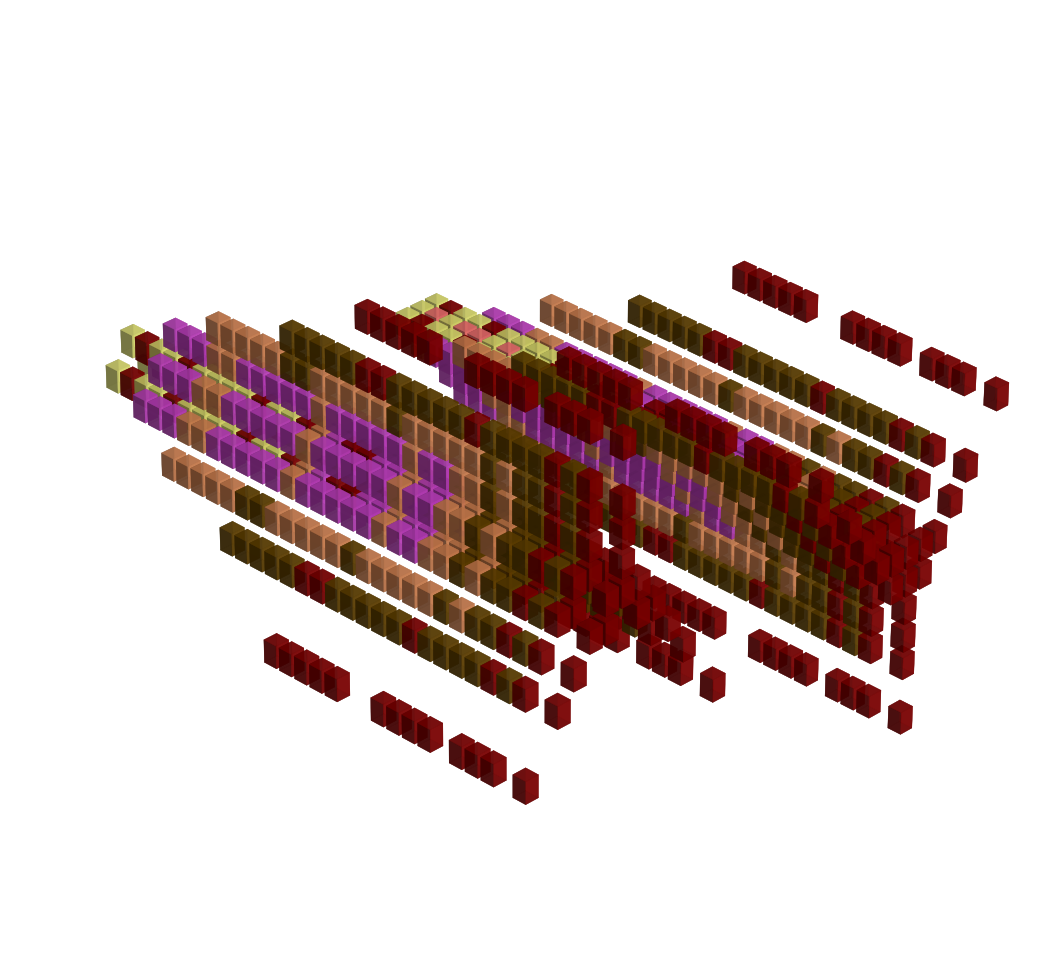
\includegraphics[width=14cm]{src/presets/pattern14-45.png}%           
    \end{adjustbox}                                                        
\caption{Evolution of Preset 15.}                                           
\end{figure}                                                               
\clearpage                                                                 
                                                                           
\begin{lstlisting}[basicstyle=\tiny,caption=Source code for Preset 15.]
preset15
        ; unusedPresetByte: Unused Byte
        .BYTE $00
        ; smoothingDelay: 'Because of the time taken to draw larger patterns speed
        ; increase/decrease is not linear. You can adjust the 'compensating delay'
        ; which often smooths out jerky patterns. Can be used just for special FX),
        ; though. Suck it and see.'
        .BYTE $03
        ; cursorSpeed: 'Gives you a slow or fast little cursor, according to setting.'
        .BYTE $01
        ; bufferLength: 'Larger patterns flow more smoothly with a shorter
        ; Buffer Length - not so many positions are retained so less plotting to do.
        ; Small patterns with a long Buffer Length are good for 'steamer' effects.
        ; N.B. Cannot be adjusted whilst patterns are actually onscreen.'
        .BYTE $1F
        ; pulseSpeed: 'Usually if you hold down the button you get a continuous
        ; stream. Setting the Pulse Speed allows you to generate a pulsed stream, as
        ; if you were rapidly pressing and releasing the FIRE button.'
        .BYTE $06
        ; indexForColorBarDisplay: 'The initial index for the color displayed
        ; in the color bar when adjusting the colors for each step.'
        .BYTE $01
        ; lineWidth: 'Sets the width of the lines produced in Line Mode.'
        .BYTE $07
        ; sequencerSpeed: 'Controls the rate at which sequencer feeds in its data. '
        .BYTE $00
        ; pulseWidth: 'Sets the length of the pulses in a pulsed stream output.
        ; Don't worry about what that means - just get in there and mess with it.'
        .BYTE $01
        ; baseLevel: 'Controls how many 'levels' of pattern are plotted.'
        .BYTE $07
        ; presetColorValuesArray: 'Allows you to set the colour for each of the
        ; seven pattern steps. Set up the colour you want, press RETURN, and the
        ; command offers the next colour along, up to no. 7, then ends. Cannot be
        ; adjusted while patterns being generated.'
        .BYTE BLACK,BLUE,RED,PURPLE,GREEN,CYAN,YELLOW,WHITE
        ; trackingActivated: 'Controls whether logic-seeking is used in the
        ; buffer or not. The upshot of this for you is a slightly different feel -
        ; continuous but fragmented when ON, or together-ish bursts when OFF. Try it.'
        .BYTE $FF
        ; lineModeActivated: 'A bit like drawing with the Aurora Borealis'
        .BYTE $00
        ; presetIndex: 'This calls in one of the 16 presets, stored Lightsynth
        ; parameters which give different effects. Try them all out io see some uf
        ; the multitude of effects which you cai achieve using the system. Some are
        ; fast, some slow, some pulse, others swirl. Play with them all, try them to
        ; different music.'
        .BYTE $04
        ; currentPatternElement: 'Initial pattern used by this preset.'
        .BYTE $04
        ; currentSymmetrySetting: 'Current symmetry setting.'
        ; Possible values are 0 - 4:
        ; 'NO SYMMETRY     '
        ; 'Y-AXIS SYMMETRY '
        ; 'X-Y SYMMETRY    '
        ; 'X-AXIS SYMMETRY '
        ; 'QUAD SYMMETRY   '
        .BYTE $04
        ; Unused Data.
        .BYTE $00,$FF,$00,$00,$FF,$00,$FF,$15,$EF
\end{lstlisting}

